\section*{Availability-led acquisition and observational velocity inversion}

This update separates live retrieval from the frozen scientific checkpoint. Availability receipts identify 26 candidate stations with public data and 8 with no data returned for the requested bands. The station list contains 51 released identifiers; its membership is not silently equated with the paper's 48 instruments. The observational scope remains incomplete.

At 2026-10-15T17:31:54.283801+00:00, stored coverage is 14,544.383 union channel-hours. Newly acquired observations contribute 1,059.305 channel-hours and 840.7 MB. These totals count actual miniSEED trace intervals, not advertised availability or queued requests. The frozen processing checkpoint uses 1,327 eligible files and 14,080.521 processed channel-hours. Later downloads are recorded separately until processed.

\subsection*{Scope, storage and availability}

The requested period is 21 January 2022 through 20 March 2025, inclusive. HH/EH channels are selected from permitted station metadata. Detailed FDSN availability, rather than earliest/latest extents, is intersected with that period and compared with the union of stored traces. The legacy ledger is classified separately; its entries are requests, not files. Whole-file checksums and trace identifiers detect duplicates; overlapping intervals count once. Existing event-selected snippets remain excluded.

The fixed reserve is 40 GiB, exceeding both the existing 20 GiB guard and 20 percent of initially free space. Retrieval keeps an additional 8 GiB above that reserve for processing outputs. The seven representative files used 74.0 MB and added 91.643 channel-hours. Their measured byte rate implies approximately 0.98 TB for remaining advertised intervals, compared with 103.0 GB initially usable above the reserve. This extrapolation is uncertain across instruments and epochs; it is updated during retrieval.

Requests use two workers, six-hour station/band cores and 30-second context. The ledger retains successful, empty, failed and pending states separately. The byte reserve is checked while streaming. Calendar-month rotation spreads coverage if storage fills. A common 1 December 2024, 00:00--06:00 UTC window is prioritized because the four public 2I stations began recording in November and were absent from training. This calendar choice does not use an earthquake catalog. A controlled collector restart and incomplete, unprocessed transfers are documented in collector\_handoff.json.

EIDA returned no requested-band availability for V0106, CDOV, CROS, CASE, V0102, V0105, V0104, CMDP. This is not proof that no recordings exist elsewhere. RAN and inaccessible local recordings remain separate deferred inputs; no credentials or restricted access were requested. Exact Calo--Tramelli values are not required for these provisional experiments and were not sought.

\par{\footnotesize\path{data/availability_extension/station_crosswalk.csv}}

\par{\footnotesize\path{data/availability_extension/response_epochs.csv}}

\par{\footnotesize\path{data/availability_extension/availability_receipts.json}}

\par{\footnotesize\path{data/availability_extension/legacy_ledger_classification.csv.gz}}

\par{\footnotesize\path{data/availability_extension/station_channel_month.csv}}

\par{\footnotesize\path{data/availability_extension/remaining_available_intervals.csv}}

The frozen cohort has 1,327 file paths, including 10 rows in byte-identical pairs. Five new downloads repeated earlier complete files while testing advertised internal gaps; they added no union coverage. Trace overlap totals 403.573 channel-hours and is counted once. The ledger subsequently excluded 88 already-successful whole-window requests, whose 0.140511 advertised gap channel-hours remain unverified. They are neither covered observations nor demonstrated absences. Fresh unattempted windows continue. Duplicate checks do not certify equality of every partially overlapping sample.

\par{\footnotesize\path{data/availability_extension/catalog_december/overlap_check.json}}

\par{\footnotesize\path{data/availability_extension/prior_success_reconciliation.json}}

\subsection*{What the expanded processing changed}

The frozen expanded checkpoint contains 256,720 picks (42,089 P; 214,631 S), 3,296 provisional associations and 31,096 assigned phases. Relative to the previous checkpoint it adds 10,052 picks. The earliest nine-file extension added 1,340 picks without changing assigned arrivals; its identity check is retained in catalog/association\_change\_check.json. Later checkpoints are distinct, and the calibration counts below are read from the selected current fit.

\par{\footnotesize\path{data/availability_extension/catalog_december/processing_checkpoint.json}}

\par{\footnotesize\path{data/availability_extension/catalog_december/association_change_check.json}}

Although assigned arrival values were unchanged, equal-time arrivals changed row order in CNV input when unrelated picks were appended. The large-cohort inversion then followed a different numerical path. Canonical event/station/phase/time sorting removes that serialization dependence; both calibration inputs now have the same checksum. The sensitivity suite was rerun after this correction. Reproducible input order does not cure the failed scientific validation.

\par{\footnotesize\path{data/availability_extension/phase_order_validation.json}}

\subsection*{Effect of the common December window}

The 1 December 2024 window has 21 stations, 63 channels and 377.977 processed channel-hours. The other five stations with availability elsewhere have no advertised data in this window. Relative to the prior catalog, 3,271 event phase sets remain identical and 25 are new or changed. Of those, 0 pass the calibration screen. Failures include 21 with fewer than four P arrivals, 23 with at most ten total phases, 18 with gap at least 180 degrees, and 3 with noncausal arrivals; categories overlap. Added provisional associations therefore do not imply improved calibration support.

\par{\footnotesize\path{data/availability_extension/catalog_december/new_association_quality.json}}

\par{\footnotesize\path{data/availability_extension/catalog_december/december_window_coverage.csv}}

\subsection*{First precision divergence}

Instrumented generic VELEST runs reproduced the saved 32-bit and 64-bit output files exactly. At iteration 3, event 1065's IV.CBAG. S ray changes between the direct and refracted branches. The preceding depths differ by 0.041 m. The next proposed depth updates are -0.496425 and 0.005972 km. A travel-time derivative change at a ray crossover therefore amplifies the arithmetic difference. This explains the first large divergence inspected; it does not prove that every later discrepancy shares that cause.

\par{\footnotesize\path{data/availability_extension/precision/ray_paths.csv}}

\par{\footnotesize\path{data/availability_extension/precision/updates.csv}}

\par{\footnotesize\path{data/availability_extension/precision/instrumentation.json}}

\subsection*{Independent profile and calendar holdout}

The inversion uses only project-generated arrivals, associations and station metadata. Initialization follows Tramelli et al. (2021), Table 1, with Vp/Vs=1.78; it is not an observed or fitted model. Fixed layer tops are -0.5, 0.5, 1 and 3 km below sea level, with a halfspace below 3 km. The poorly sampled 10-km interface is omitted. P and S velocities subsequently vary independently. Zero station corrections initialize the fit; the best-observed training P station fixes the reference. P and S weights are 1 and 0.5. Generic VELEST clips nonpositive source depth and may reset a boundary source to 0.1 km; this is a solver convention, not an observed depth floor.

Prelocation uses 21 iterations, followed by velocity-only and joint velocity/location/station-correction stages and three further convergence blocks, each of 14 iterations. Holdout locations are optimized for 35 iterations with model and corrections fixed. Origin, horizontal, depth, velocity and station damping are 0.01, 0.10, 0.10, 1.0 and 0.10; layer damping is 10. Maximum depth and velocity updates are 0.2 km and 0.1 km/s. Smaller steps and stronger location damping address the observed ray-crossing sensitivity; these are disclosed alternatives, not recovered Tan settings. The existing 100 m location, 0.05 km/s velocity and 0.02 s correction stability gates are retained.

46 training events contain 709 arrivals and span pre-2025 days; at most 20 chronological events per day balance the dominant May 2024 swarm. All 62 eligible 2025 events, with 1,065 arrivals, are excluded from velocity/correction fitting. The holdout is separated in time, rather than selecting every fifth event within a swarm. Holdout origin times and locations remain nuisance fits, so this is a conditional travel-time test, not absolute location validation.

The balanced fit lowers training RMS from 0.2082 to 0.1759 s, but increases holdout RMS from 0.2406 to 0.2778 s. Using all 490 training events has final iteration-change gate result False, and holdout RMS is 0.2727 s. Neither fit is accepted. Starts scaled by +/-10 percent, 32-bit arithmetic, event selection and a 0.1-km depth-step limit were actually run. Sensitivity ranges are not confidence intervals.

The balanced holdout has 186 arrivals in 15 station/phase pairs absent from training. Their fitted RMS is 0.3966 s. For observed training pairs, fitted holdout RMS is 0.2454 s versus 0.2331 s initially. The failure therefore cannot be explained only by the missing stations. The smallest targeted extension is simultaneous pre-2025 recordings that supply those station/phase pairs, followed by arrival review and a still-separated holdout. A sufficient event count cannot be established from the current fits.

\begin{center}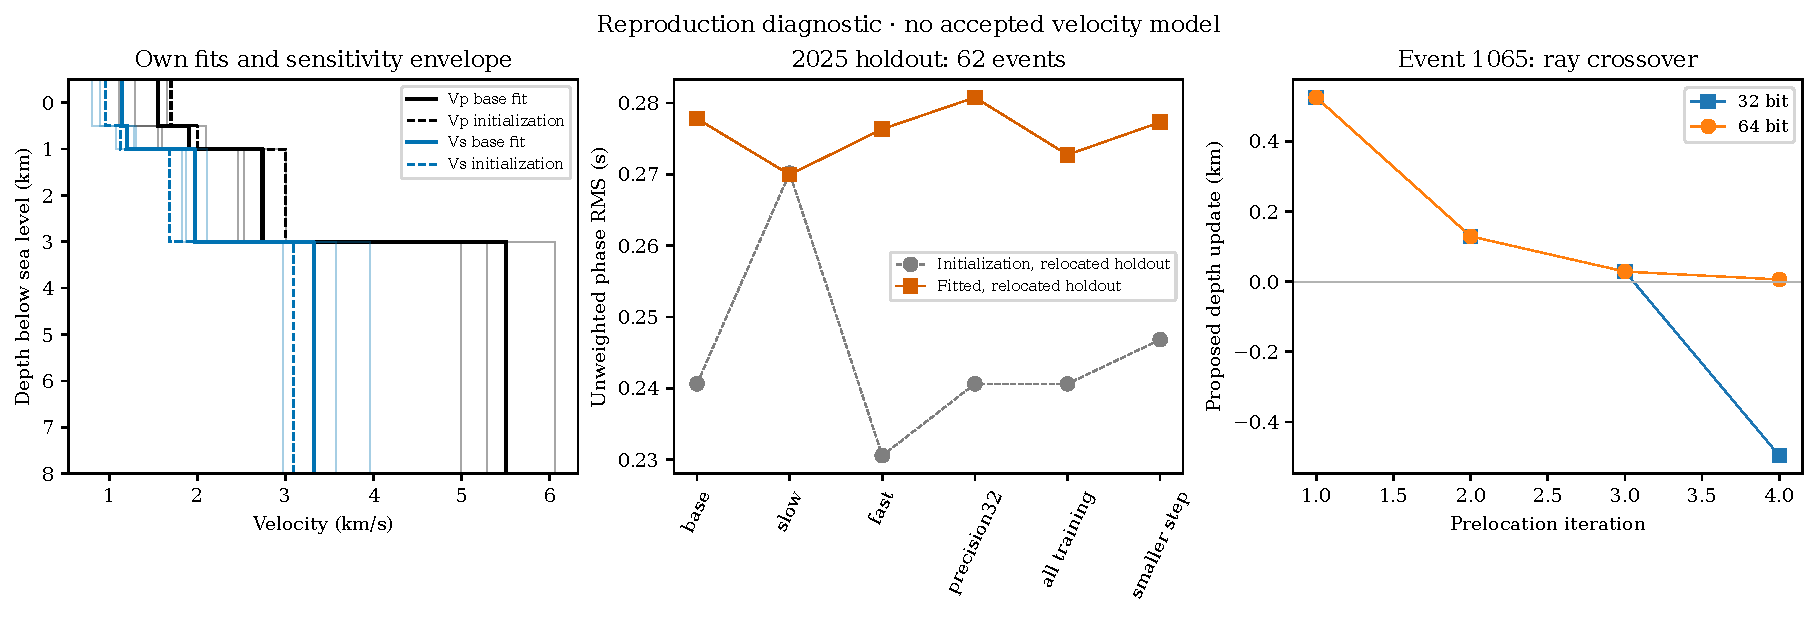
\includegraphics[width=\linewidth]{figures/observational_velocity_diagnostic.pdf}\end{center}

Reproduction diagnostic, not a publication panel. Dashed velocities are initialization; solid curves are independent provisional fits. The spread summarizes six specified sensitivity experiments. All residuals and depth steps are saved numerical results.

\par{\footnotesize\path{data/availability_extension/velocity_december/summary.json}}

\par{\footnotesize\path{data/availability_extension/velocity_december/sensitivity_profiles.csv}}

\par{\footnotesize\path{data/availability_extension/velocity_december/holdout_station_phase.csv}}

\par{\footnotesize\path{data/availability_extension/velocity_december/summary.json}}

\subsection*{Downstream scope and panel status}

The expanded cohort was also located in five fixed-model passes using the independently fitted base trial, with the documented 0.4/0.3 s residual rejection and final numerical filters. 1,414 of 3,018 initial causal events pass those filters. Figure S6 displays this unaccepted sensitivity calculation. Its model fails the holdout test; it is not promoted to a validated catalog. The earlier two-round fixed-grid relocations, magnitudes and mechanisms retain their earlier model and cohort and remain provisional.

\par{\footnotesize\path{data/availability_extension/catalog_december/locations_canonical/summary.json}}

Figures 2--4 and S7--S15 continue to identify their preserved numerical checkpoint unless an explicitly updated panel is listed. More raw files or isolated picks do not establish additional events, improved depths, completeness or reliable mechanisms. No published result table, catalog, pick, fitted velocity or digitized value fills a gap. Published figure images remain confined to the comparison PDF.

\subsection*{Rebuild and resume}

Use \path{scripts/rebuild_availability_extension.py} to verify the saved numerical checkpoint, regenerate its plots and compile both existing PDFs. Scientific commands and input placement are listed in \path{docs/AVAILABILITY_EXTENSION.md}. Acquisition and incremental picking have separate receipts; they are not counted as completed catalog analysis.

Earlier data/eida\_continuation and its plots remain preserved. The main manuscript, supplement, comparison layout, status record and document products are updated from saved results. Failed models and the original precision runs are retained. Reproduction remains partial; no panel is promoted to fully reproduced by this update.


\section{Current EIDA processing and validation}

The current eligible continuous-observation checkpoint contains 246,668 picks and 3,271 provisional associations from 1,285 files and 13,467.933 channel-hours. 2996 associations have causal usable arrivals; 552 meet the numerical calibration selection. 1435 locations pass VELEST filters and 1050 remain after both TomoDD rounds and the gap filter. All known event-selected snippets are excluded. These calculations remain provisional; filter passage does not establish correct event identity or fault geometry.

Relative to the preserved previous checkpoint, retained trial events increased from 123 to 1050. Conditional SVD estimates increased from 80 to 352; median vertical uncertainty changed from 233.4 to 244.6 m and the maximum from 1336.6 to 3499.1 m. The cohorts differ, so these changes do not establish improved location accuracy. Current depth quantiles and year counts are saved in result\_summary.json; no accepted caldera geometry or depth limit is inferred.

New requests: {'downloaded': 275, 'no\_data': 1}; 3.481 GB returned. 73,641 requests remain unattempted; this is unfinished acquisition, not a remote-access failure. The batch prioritizes final study days, then calendar-selected dates across years. An additional 20-station batch covers the full 2024-05-20 18:00 to 2024-05-21 00:00 UTC interval containing the S4 benchmark. This purposeful continuous-window sampling does not establish discovery of the known swarm or population completeness. Original files, checksums and request outcomes are saved. RAN access and the exact Calo--Tramelli profile were deferred as instructed.

\par\path{data/eida_continuation/request_ledger.csv.gz}\par\path{data/eida_continuation/station_coverage.csv}\par\path{data/eida_continuation/unobserved_channel_intervals.csv}

Response epochs cover 13467.933 observed channel-hours; 0.000000 hours lack complete responses. The 14 event-selected files remain preserved for labeled waveform checks; they do not supply independent continuous detections or completeness statistics.

The 165 original baseline files retain their earlier 15-second inference margins; new segmented inference uses 30 seconds. Original waveform, configuration and saved-pick hashes were verified. Known event-selected windows are excluded from both detections and exposure. Reduced station count relative to the previous checkpoint reflects that exclusion, not loss of downloaded continuous records.

\subsection*{Location validation}

The unconstrained new-cohort fits had negative isotropic bulk modulus in the 3--5 km layer (Vp/Vs 1.073 and 1.088). Those outputs and the interrupted relocation attempt are preserved in unconstrained\_calibration.zip. The current fit uses one disclosed increase to uniform velocity-layer damping 100, motivated by that failure and generic VELEST regularization guidance. No observations or acceptance limits changed. The resulting velocities are strongly influenced by the starting grid; physical admissibility does not establish data resolution or exact reproduction.

Calibration dates: {'2022-01-21': 1, '2022-01-24': 2, '2022-01-25': 1, '2022-01-26': 2, '2022-01-28': 1, '2022-02-01': 2, '2022-03-01': 1, '2023-03-01': 6, '2024-02-01': 9, '2024-04-01': 1, '2024-05-20': 464, '2025-01-01': 1, '2025-02-01': 6, '2025-03-18': 24, '2025-03-19': 14, '2025-03-20': 17}. The chronological every-fifth-event holdout is interleaved within the sampled swarms; it is not an independent out-of-region or out-of-period accuracy test.

Separating fixed-model events into batches was rejected after a 1.91 km maximum depth change. Production retains global VELEST updates. A zero-term Cholesky optimization reproduced six complete 552-event, 9,529-phase runs byte for byte, including location, velocity, station-correction and residual files. A further 32-bit dense comparison of current fixed-model prelocation is also byte-identical. Both arithmetic precisions use this checked optimization. Numerical equivalence is distinct from accuracy.

TomoDD storage was expanded to accommodate the measured phase pairs. Zero-correlation diagnostic logging errors in generic TomoDD and HypoDD were corrected without changing inverse equations. The first TomoDD cluster remained byte-identical through all eight iterations; a successful HypoDD component also remained byte-identical. The repaired small SVD component returned three additional estimates; the component rejected as airquakes was not forced to return a solution.

\par\path{data/eida_continuation/tomodd_logging_fix_check.json}\par\path{data/eida_continuation/hypodd_logging_repair.json}

\par\path{data/eida_continuation/sparse_check.json}\par\path{data/eida_continuation/unconstrained_archive.json}\par\path{config/eida_calibration.json}

Full precision paths differ by 1075.2 m horizontally and 0.850 km in depth; precision gate: False. Regional-start depth difference: 1.520 km. Held-out refitting uses 441 training and 111 withheld events. Held-out RMS changes from 0.2403 to 0.2081 s.

TomoDD inter-round maximum change is 1830.3 m horizontally and 1.154 km vertically. 404 retained events have no waveform-correlation links. SVD errors are conditional on the fitted model and phase assignments, and exclude these systematic uncertainties. Generic HypoDD also clips the negative CFB1/CFB3 elevations to sea level, omitting 40.4/38.7 m of receiver depth; the original metadata and this approximation are recorded in receiver\_convention\_check.json. The corrected S9 threshold is $>$=100, following the supplement's exclusion of sums below 100; no gate was weakened to create a result.

Compared with the previous 123-event trial, the current trial has 1050 events. Reciprocal origin-time matching ($<$2 s, no author catalog) links 22 events. This is a change diagnostic, not an accuracy measurement. Independent S--P checks use 4368 measurements with RMS discrepancy 0.1820 s against the own approximate model.

The precision runs use identical observations, initial files and controls. A 150 m maximum depth difference already occurs during fixed-model prelocation. The final median difference is 40 m and the 95th percentile is 273 m, with a maximum of 850 m. Common intermediate starts reduce some differences but do not remove them. The exact ill-conditioned mode or ray switch was not isolated, and these differences are not treated as harmless rounding.

\par\path{data/eida_continuation/precision_diagnosis.csv}

\par\path{data/eida_continuation/calibration/merged4/heldout/summary.json}\par\path{data/eida_continuation/calibration/merged4/validation.json}\par\path{data/eida_continuation/calibration/merged4/uncertainty/summary.json}

\subsection*{Template and frequency-index screening}

1843 unconfirmed template-score crossings over 140.656 common CAAM/COLB hours. Twelve highest scores per template displayed from original waveforms with measured frequency indices and amplitude ratios. No confirmed cluster or accepted hybrid magnitude. AI inspection of 36 displayed crossings found 4 preceding-packet tails and 3 ongoing-activity windows; the other transients remain unclassified. No human review.

\par\path{data/eida_continuation/hybrid/provenance.json}\par\path{data/eida_continuation/hybrid/visual_review.csv}

The written-method template times select original waveform examples only. These templates never enter the continuous detection catalog or exposure. Other score crossings remain unreviewed; no verified three-year hybrid chronology or family magnitudes are available.

Phase support in the retained relocated set: {'events': 1050, 'no\_P': 5, 'fewer\_than\_four\_P': 396, 'no\_S': 0, 'P': 5225, 'S': 8079}. S-only or P-poor associations have weak independent control on origin time and absolute depth. The published six-pick gate is retained; these diagnostics are disclosed rather than silently adding a new selection.

\subsection*{Mechanisms}

Before visual review, automatic first-motion screening evaluated 197 events and 1969 station windows; 12 events had at least eight stable automatic signs. The unchanged SKHASH geometry gates returned 0 mechanisms. These automatic signs are not counted as visually reviewed measurements.

12 unaccepted own FK/gCAP trial fits using newly available EIDA records and the current own model and explicitly linked own candidate geometry. 99 AI-reviewed polarities, 108 AI-reviewed ratios; no human review. SKHASH returns 2 solutions. Low-band variance reduction 1.3--14.4\%; orientations change 45.0--95.0 degrees between frequency bands. Gray beachballs denote unvalidated trials; background is the new independent catalog, never joined to candidates by integer ID. SKHASH returns 2 quality-D trials. No scientifically accepted mechanism.

\begin{center}\small\begin{tabular}{rrrrl}\toprule Candidate & P & S/P & Azimuth gap & Requirement\\\midrule

212 & 3 & 5 & 175.5 & Fewer than 8 P\\

312 & 5 & 5 & 155.9 & Fewer than 8 P\\

315 & 4 & 4 & 252.9 & Fewer than 8 P\\

359 & 4 & 8 & 165.4 & Fewer than 8 P\\

373 & 3 & 5 & 177.8 & Fewer than 8 P\\

649 & 8 & 10 & 120.5 & Geometry/model validation\\

698 & 1 & 1 & 360.0 & Fewer than 8 P\\

815 & 4 & 6 & 167.1 & Fewer than 8 P\\

100331 & 16 & 12 & 103.6 & Geometry/model validation\\

100946 & 17 & 13 & 95.3 & Geometry/model validation\\

100948 & 0 & 0 & 360.0 & Fewer than 8 P\\

101038 & 11 & 15 & 90.3 & Geometry/model validation\\

101400 & 14 & 16 & 83.6 & Geometry/model validation\\

101760 & 9 & 8 & 84.0 & Geometry/model validation\\

\bottomrule\end{tabular}\end{center}

\par\path{data/mechanism_eida/review_transfer.json}\par\path{data/mechanism_eida/review_decisions.csv}\par\path{data/mechanism_eida/skhash.log}\par\path{data/mechanism_eida/gcap_band_sensitivity.csv}

Prior review decisions are retained only after explicit observation-window equality checks; new or changed windows receive a separate AI review record. Zero human reviews are claimed. Candidate labels preserve earlier review IDs; the shared-phase mapping identifies current locations and explicitly marks any retained historical location. The new model and all locations remain provisional. Event-dependent filters and source controls are exploratory; neither weak fits nor a returned solver file establishes a reliable mechanism.

\begin{center}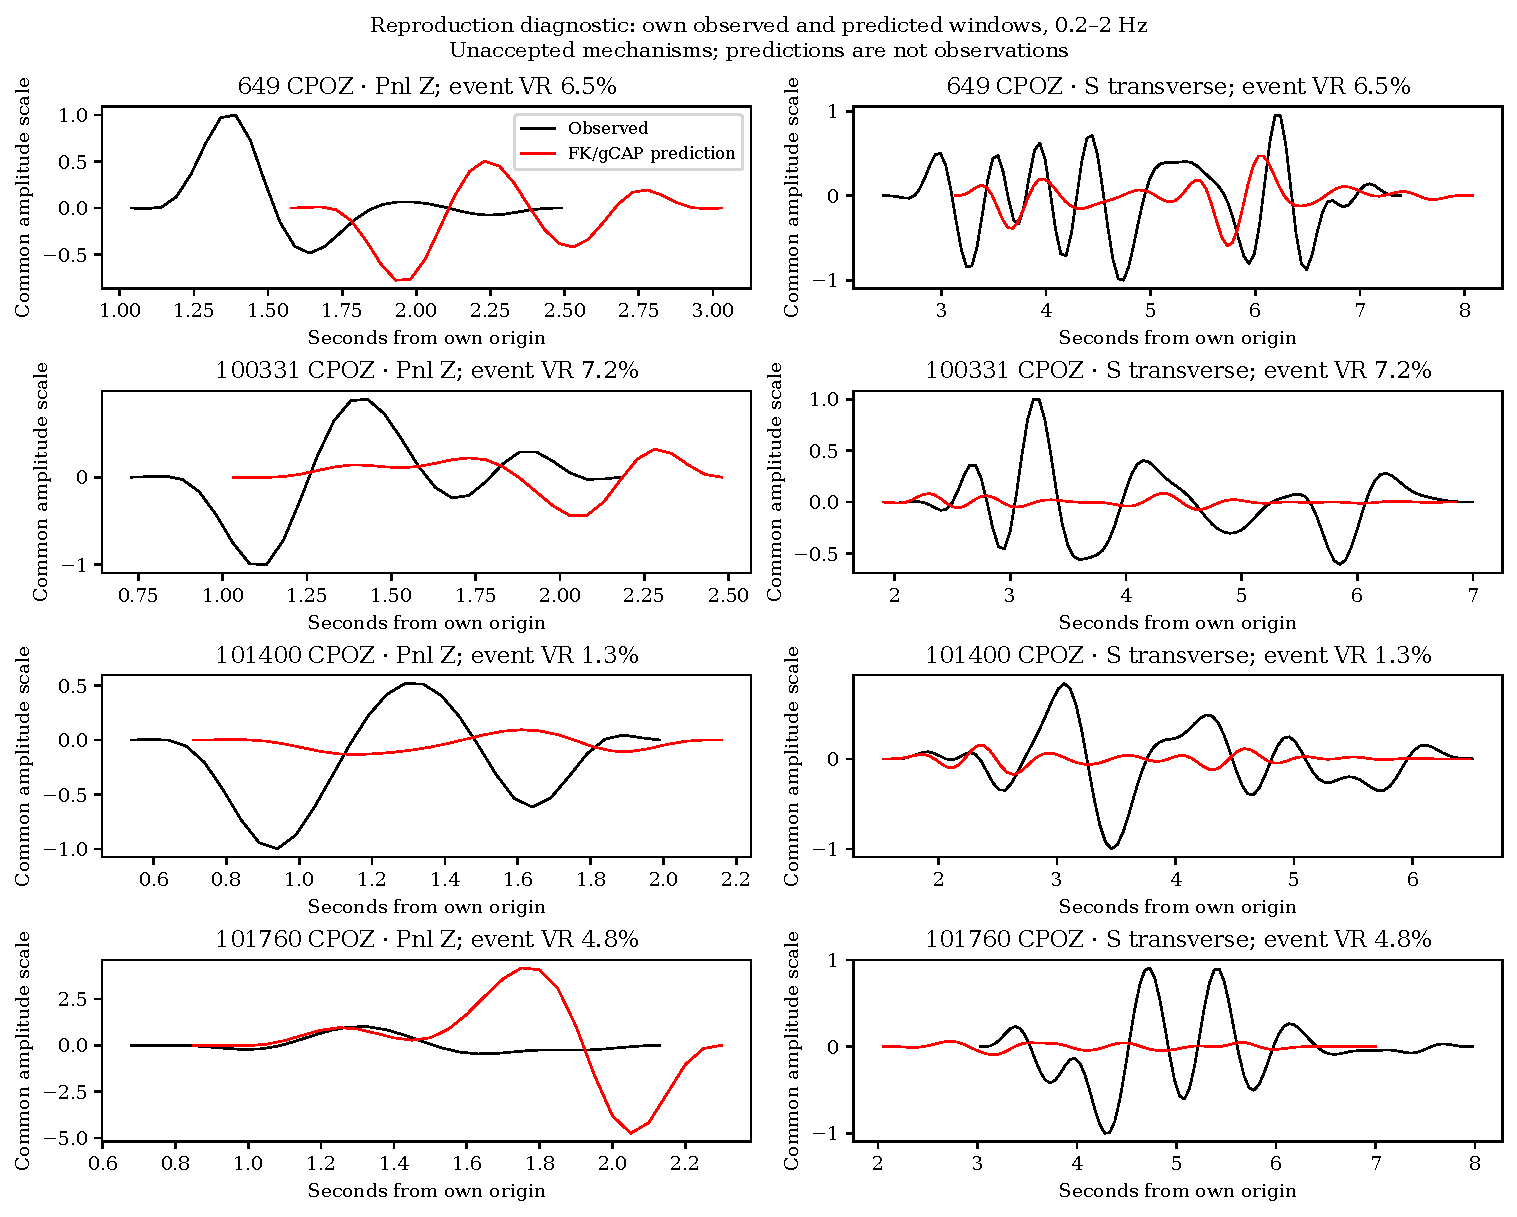
\includegraphics[width=.95\linewidth]{figures/mechanism_eida_fit_diagnostic.pdf}\end{center}

Reproduction diagnostic, not a publication figure. CPOZ observations and own FK/gCAP predictions for four explicitly selected trial events share one amplitude normalization per pair. Red curves are theoretical predictions, not observational or synthetic fixture data. Predicted amplitudes are not normalized separately. Saved fitted lags are included; weak event variance reduction and band dependence prevent mechanism acceptance.

Own SKHASH--gCAP Kagan angles span 35.6--79.1 degrees across 4 event/band pairs. These trial comparisons do not establish the paper's high-quality selection because locations, phase identity and model sensitivity remain unresolved.

\par\path{data/mechanism_eida/skhash_gcap_comparison.csv}\par\path{data/mechanism_eida/candidate_requirements.csv}

Eight additional downstream-only P arrival marks were inspected against raw and response-corrected traces; seven first-motion signs were retained. CPOZ supplies three additional clear P/S packets. These AI arrivals do not enter the detection or association catalog. Candidate 100948 has unresolved identity amid preceding activity, about 14 seconds after a larger candidate; all its amplitude measurements fail quality control. Near/pre-origin CAAM/COLB motion for candidate 101760 flags an association/origin inconsistency. Neither candidate is silently removed or accepted as a validated event.

\par\path{config/mechanism_eida_arrivals.csv}\par\path{data/mechanism_eida/new_visual_review.json}\par\path{data/eida_continuation/catalog_quality_flags.csv}

\subsection*{Rebuild and preserved checkpoints}

Run \texttt{.venv/bin/python\allowbreak{} scripts/rebuild\_eida\_followup.py\allowbreak{} --analysis} for the frozen observation set, or omit \path{--analysis} to verify saved numerical files and rebuild figures and both PDFs. Retrieval is separate: \texttt{.venv/bin/python\allowbreak{} scripts/collect\_eida\_followup.py\allowbreak{} --max-jobs\allowbreak{} 256\allowbreak{} --workers\allowbreak{} 4}. It selects only pending, never-attempted requests. The command does not retry prior empty or failed intervals. Actual execution and build outcomes are in \path{data/eida_continuation/pipeline_execution.json} and \path{data/eida_continuation/rebuild_result.json}.

Earlier data/local\_extension, data/coverage\_extension and data/mechanism\_followup remain preserved, with their distinct identifiers and superseded figures. The main report, comparison PDF, panel records and current figure fragments are updated; no published-result tables enter the calculation. Existing historical/context, training-example and original-region-mask limitations are unchanged.

\subsection*{Current panel summary}

Partial: 1A, 1B, 1C, 2A, 2B, 3/map, 3/northing-depth, 3/easting-depth, 4A, 4B, S1, S2, S4A, S5/map, S5/northing-depth, S5/easting-depth, S6/map, S6/northing-depth, S6/easting-depth, S7A/map, S7A/easting-depth, S7B, S7D, S7F, S7C, S7E, S7G, S8A, S8B, S10/2022, S10/2023, S10/2024, S10/2025, S11/swarm-1, S11/swarm-2, S11/swarm-3, S12A, S12B, S12C, S12D, S12E, S12F, S12G, S12H, S13A, S13B, S14/1, S14/2, S14/3, S15A, S15B, S15C, S15D. Unreproduced: S3A, S3B, S3C, S3D, S4B, S9/map, S9/northing-depth, S9/easting-depth, S11/swarm-4, S14/unclustered. No full independent reproduction is claimed.


\section*{Preserved earlier checkpoint records}
The following records retain earlier cohort-specific counts, methods and failures. They are historical evidence, not the current coverage totals or an additional catalog.

This record describes the current continuation, not the superseded nine-event run. Historical outputs remain recoverable from Git. The main paper and reproduced supplement contain only corresponding publication panels; published images occur only in the separate comparison PDF.

\section{Local-file continuation and mechanism measurements}
This continuation supersedes the current scientific figures for 2--4, S1, S6--S8 and S10--S13. Previous data and plots remain in their labeled cohort directories. No earlier event identifier is silently reused in the new cohort. All new empirical points come from observed waveforms and this implementation's saved calculations; theoretical FK Green functions are predictions, not observations. Published images occur only in the separate comparison PDF.

\paragraph{Inputs and actual processing.}
Fourteen previously omitted files were processed: six original CAAM/COLB template windows, seven short local-archive records, and the original CSOB benchmark window. These event-selected observations do not measure continuous discovery exposure. Twenty previously unattempted public requests were issued: 19 returned readable files and one CPIS interval returned HTTP 204; zero failed and no previously attempted interval was retried. All 33 files entered PhaseNet. Compatible older per-file inference and day-association results were reused only after observation, model and settings checks. Raw observation hashes, short-window classifications and processing receipts are in \path{data/local_extension}.

The new checkpoint has 1,024 files, 30 station names, 87 channels and 8,952.452 union channel-hours, an increase of 245.482 hours. Four added names occur only in short single-channel records. Response epochs cover 8,952.386 hours; four short intervals totaling 0.0667 hours lack valid responses. Ten picks at CROS, V0102 and V0105 lack verified association metadata and remain in \path{picks_without_metadata.csv}. The independent selection contains 136,376 picks, 7,416 associated picks and 1,024 provisional events. Requests with no returned observations are not exposure. The frozen queue has 842 downloads, 36 empty responses, 11 failures and 73,917 pending requests. Full study-period coverage remains unfinished. The alternative Tramelli (2021) association profile is retained and explicitly prevents an exact starting-model claim.

\paragraph{Calibration and relocation outcomes.}
All nine requested calibration/downstream stages exited successfully; scientific acceptance is false. The new 921-event causal input supplies 38 numerical calibration candidates, 219 VELEST filter passes and 123 final relocated gap passes. Two fixed-grid TomoDD rounds, 80 conditional SVD estimates, 67 provisional amplitude magnitudes and 122 CPOZ component gathers were recomputed for this cohort. On 398 shared waveform differential observations, residual RMS decreases from 0.04125 to 0.03940 s; on 4,367 shared picked differences, from 0.10738 to 0.10130 s. The maximum between-round shift is 386 m horizontally and 0.372 km vertically. Thirty-four retained events have no cross-correlation link and none has more than 100. S9 therefore still has no qualifying result.

Full 32/64-bit calibration paths differ by 558 m horizontally, 0.89 km in depth, 0.32 km/s in velocity and 0.25 s in station delay. Identical converged starts give identical printed coordinates and velocities; this does not remove accumulated nonlinear sensitivity. Regional-start depth differences reach 1.04 km. Earlier instrumentation and failed held-out validation are retained as historical evidence, not asserted to have been rerun for this extension. The new association at 29 January 2022 06:26:03.080 UTC has one P and five S picks. Its reported VELEST RMS increases 0.44, 0.45, 0.46 s in the first three passes; residual rejection leaves too few picks, so it does not survive. The final 123 origins match the prior cohort, with coordinate differences at most 0.001 km vertically. More input did not yield another accepted or retained event.

The relocated-subset magnitude inversion uses 5,887 measured channels, 1,623 SNR passes and 884 relative-amplitude equations. Routine duration magnitude is a documented external calibration prior. Conditional $M_c=0.0$ and $b=0.866\pm0.110$ describe 41 selected magnitudes, not population completeness. There are 383 positive observed S--P pairs, with 0.1777 s RMS against the approximate own model; 42 deep events are flagged for review. These checks do not validate absolute depths.

\paragraph{Polarity and amplitude review.}
The frozen eight-event candidate set preserves the requested event 649 identifier. All 180 available station-event records were inspected visually by the AI; none was reviewed by a human seismologist. Responses verify the upward vertical orientation. First motions were read from counts and response-corrected velocity without an additional bandpass. Accepted and rejected judgments, trace references and reasons are saved in \path{data/mechanism_followup/review_decisions.csv}. Some initially assigned signs describe later lobes rather than first motions and were corrected. The 13 additional stations for 649 were inspected: CGAU, CLAC, CSOC, CBAG, CCAP, CFMN, CMSN, CMTS, COLB, CPIS, CQUE, CRUS and CUMA. The new AI-reviewed CFMN P arrival is 20 March 2025 06:32:18.910 UTC, with approximately 0.03 s reading uncertainty; it is not an author pick.

S/P is the ratio of peak three-component velocity norms in independently aligned P and S windows, filtered 1--15 Hz. P uses P to min(P+0.30,S-0.10) s, S uses S to S+0.50 s; noise uses P-3 to P-1 s. Both peak/noise-RMS ratios must exceed three. Of 61 automated measurement passes, 41 retain visually usable phase packets; 29 first motions survive AI review. These explicit exploratory windows are not asserted to recover Tan's unpublished per-event choices. Seven events have fewer than eight reliable polarities. Event 649 has eight, but SKHASH's computed azimuthal gap is 96.57 degrees, above the unchanged 90-degree limit. The successful software run returns zero solutions, not a negative finding about faulting style.

\paragraph{FK and gCAP trials.}
Official generic FK 3.3 and Zhu's generic gCAP source were inspected and compiled; archive examples, example results and plotting scripts were excluded. Source URLs, archive hashes and extracted member lists are in \path{data/mechanism_followup/method_resources.json}. The gCAP distribution requires unavailable Numerical Recipes and SAC filtering functions. A separately named port replaces its three-dimensional curvature eigensolver with a Jacobi calculation and filters complete observations/Green functions externally before fitting. The fixed-matrix eigensolver check differs from NumPy by at most $6.7\times10^{-8}$; this is a software test, not an empirical result. External filtering differs from stock segment filtering and limits exact reproduction.

Seven candidates supply at least four reviewed three-component stations; 698 supplies only one. FK generates nine double-couple components per station using the independently fitted four-layer provisional model. Depth is below sea level, with the model surface at $-0.5$ km; source depth is shifted by +0.5 km. Individual receiver topography is not corrected. Density uses the documented FK fallback $\rho=0.77+0.32V_p$ in g/cm$^3$; $Q_S=500$, $Q_P=1000$ are defaults, not measured properties. Verified components rotate to up, outward radial and counterclockwise transverse in cm/s. Horizontal-energy consistency passes.

Both frequency trials use fixed own locations/depths, a 10-degree double-couple grid, 0.1 magnitude increments and a 0.2 s source duration. Pnl windows are P-0.3 to P+1.2 s; surface-wave windows S-0.3 to S+4.7 s, with maximum shifts 0.5 and 1 s, Pnl weight two and distance exponents one and one-half. These are disclosed assumptions. The two bands are 0.2--2 and 1--5 Hz. All seven fits return finite numerical outputs, but variance reduction remains poor and orientations are strongly frequency-dependent. No solution is accepted; no SKHASH--gCAP comparison can be computed without a SKHASH solution. The rotation below compares two own gCAP trials only.

\begin{center}\small\begin{tabular}{rrrrrr}\toprule Event & P signs & S/P & VR low (\%) & VR high (\%) & Rotation ($^\circ$)\\\midrule
212 & 3 & 5 & 6.9 & 7.1 & 79.0\\
312 & 5 & 5 & 11.9 & 7.0 & 73.7\\
315 & 4 & 4 & 14.8 & 6.4 & 97.9\\
359 & 3 & 7 & 7.3 & 3.9 & 48.3\\
373 & 2 & 4 & 3.9 & 5.0 & 34.2\\
649 & 8 & 10 & 6.0 & 4.2 & 79.1\\
698 & 1 & 1 & --- & --- & ---\\
815 & 3 & 5 & 9.2 & 2.3 & 80.6\\
\bottomrule\end{tabular}\end{center}
Event-specific requirements, logs, controls, observed SAC inputs, theoretical Green functions and fitted traces are retained under \path{data/mechanism_followup}. For 649, another reliable first motion in the uncovered sector or justified review of current ambiguous onsets is required even to pass the SKHASH gap gate. Additional stations are not automatically usable polarities. For every other candidate the insufficient polarity count is recorded explicitly. Accepted waveform mechanisms further require defensible source locations/model, reviewed windows and stable fits; an optimizer returning angles does not establish these conditions.

\begin{figure}[H]\centering
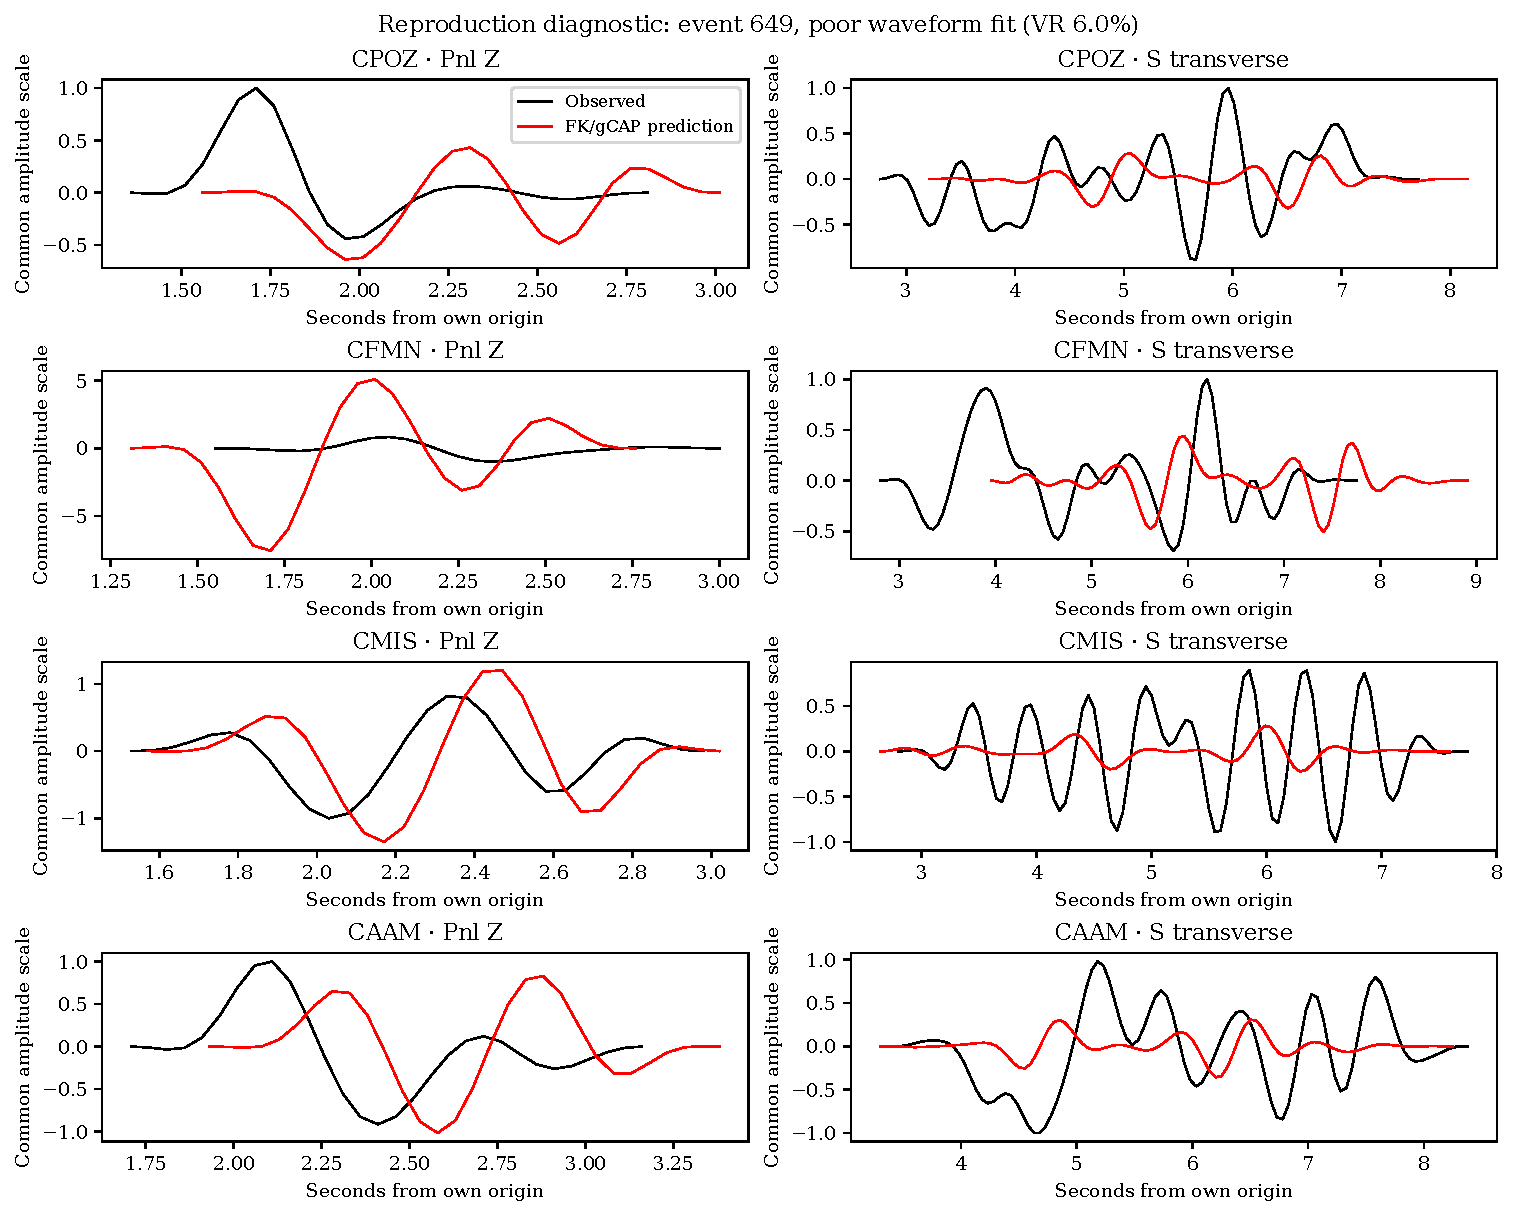
\includegraphics[width=.97\linewidth]{figures/mechanism_fit_diagnostic.pdf}
\caption{Reproduction diagnostic, not a publication figure: event 649 observations and FK/gCAP predictions at four stations. Each pair shares the observed-peak amplitude normalization; the prediction is not normalized separately. Pnl and transverse-S discrepancies explain why the trial beachball is unaccepted.}
\end{figure}

\paragraph{Rebuild, provenance and replacements.}
Run \path{.venv/bin/python scripts/rebuild_local_followup.py} to validate saved manifests, redraw these panels, integrate their records and compile both documents. The option \path{--analysis} reruns the frozen inference/association, calibration/downstream stages and mechanism calculations from retained observations; it does not download a new waveform batch or replace AI review with an automatic claim of human review. Successful commands from this continuation are recorded in \path{data/local_extension/execution.json} and mechanism execution logs; old inference caches were hash-checked, not recomputed from scratch. The original waveform inputs remain local with source receipts and hashes. The source and result files superseded in the current documents are listed in \path{docs/local_followup.md}; historical numerical cohorts remain unchanged.


\section{Scientific specification and input verification}
The local main paper and supplement were read before changing scientific outputs. Main captions 1--4, supplementary captions S1--S15 and the methods are readable. The two uploaded ZIP archives were listed and CRC-tested without executing their contents. Their exact filenames, sizes and checksums remain in the input inventory.
\begingroup\small\begin{longtable}{p{.52\linewidth}r p{.25\linewidth}}
\toprule
File & Bytes & Inspection\\\midrule
\endhead
\path{tanmodel.pdf} & 2140554 & Text and captions readable\\[3pt]
\path{tanmodelsupp.pdf} & 62164947 & Text and captions readable\\[3pt]
\path{science.adw9038_data_s1_to_s3.zip} & 12960255 & Directory readable; CRC passed; not executed\\[3pt]
\path{science.adw9038_interactive_plot_s1.zip} & 8852485 & Directory readable; CRC passed; not executed\\[3pt]
\bottomrule
\end{longtable}
\endgroup
Data S1 is the authors' derived catalog, S2 their associated phases, and S3 their focal mechanisms. The second archive contains an interactive derived-result visualization. None supplies original waveform observations for the independent workflow. These products are excluded from initialization, filtering, calibration, tuning and plot filling. The current workflow does not read these derived tables or compute result-table comparison statistics. Earlier comparison products are quarantined. Published reference images are used only in the separate comparison PDF.

The user now expressly permits the external routine catalog for Figures 1A, 1C and S5, and for the paper's documented duration-magnitude regularization. Those roles are implemented separately from picking and association. Released trained PhaseNet weights, generic method software, original observations and required metadata are permitted. The Tan-fitted 1D model and station corrections, event results, picks and study-specific scripts remain excluded. No figure was digitized or used as numerical input.

\section{Data access and actual coverage}
The access refresh found readable miniSEED examples for seven station codes in the temporary archive: CFB1, CFB3, CROS, CRUS, V0102, V0105 and CMDP. CRC, decompression, sample headers and hashes were checked using bounded HTTP ranges; nothing was executed. The saved directory contains 319,889 miniSEED members but no CGAU, CLAC, CREM or CSOC member, although these four names appear on the index page. The original access checks have now entered the explicitly labeled local-window picking pass. They are event-selected observations, not continuous exposure. Their author-event-selected windows and unresolved station epochs prevent treating this archive as an unbiased discovery record. Exact receipts are in \path{docs/local_waveform_receipts.json}.


\begin{longtable}{p{.70\linewidth}r}\toprule Quantity & Observed result\\\midrule\endhead
GNSS observations in plotted interval & 8743\\
GNSS extension in 2025 (days) & 79\\
GNSS overlap RMS after offset (m) & 0.000295\\
All historical routine records & 26425\\
Located historical routine records & 16046\\
Located routine study events & 12503\\
Difference from published study count & 420\\
Processed waveform files & 318\\
Processed union channel-hours & 2955.824\\
Merged picks & 63036\\
Provisional GaMMA events & 740\\
Downloaded six-hour chunks & 144\\
Pending six-hour requests & 74301\\
\bottomrule\end{longtable}

The study interval is 21 January 2022 through 20 March 2025, with the exclusive endpoint 21 March. The previous full-span HTTP 413 responses were request-size failures, not evidence of unavailable observations. The collector queries FDSN availability and requests six-hour intervals plus half-hour calendar checks with 30-second processing margins. The smaller checks sample the full study date range without implying continuous coverage. Every successful miniSEED response is read, identified by network/station/channel, clipped to its core and hashed. Overlapping channel intervals are merged before computing channel-hours. The original full-period queue contains 74,445 six-hour requests; 229 half-hour calendar checks were added across quarter starts and the study boundaries; unattempted and failed requests never count as coverage. The portable checkpoint and per-request receipts distinguish completed downloads from the pending multiyear workload. At this checkpoint the full period has not been retrieved or processed. The raw inventory includes six original recordings selected for the written-method hybrid templates. These event-selected original windows now also enter the separately labeled local picking pass; their selection cannot establish unbiased continuous discovery. No author-derived pick or event solution is used. Thus raw observation coverage is not identical to inference exposure.

The collector resumes from \path{inputs/continuation/acquisition.sqlite}, uses six concurrent transfers and stops if shared free space falls below 20 GiB. Linear extrapolation from this download batch gives roughly 970 GB for the entire queue, against about 152 GiB free when checked. That estimate varies with compression and coverage and is not a measured full-archive size. Streaming processing with separate retention or additional storage is needed for the whole queue; pending work is labeled unfinished acquisition, not remote inaccessibility. Processing hours refer to successfully read input channels. Short fragments and missing components can prevent PhaseNet output, and these hours are not claimed as complete three-component detection exposure. The phase-classification warnings are retained in execution logs.

Fresh response-level StationXML was obtained for 22 IV stations and four 2I stations, including historical epochs. Public IT response queries returned HTTP 204. Eight additional IV identifiers missing from the XML---V0106, CDOV, CROS, CASE, V0102, V0105, V0104 and CMDP---were checked individually for full-period availability; all returned HTTP 204. A subsequent all-network StationXML query for these eight codes also returned HTTP 204. These are service-specific no-data responses, not proof that local or author-held records do not exist. RAN's login page explicitly requires registration or credentials to download SAC/ASCII waveforms; those credentials are unavailable. This is an access limitation, not a prompt restriction. Public RAN metadata were subsequently obtained directly from its station directory and XML download: all 17 candidate station files are readable, with 57 study-overlapping HN/HG response epochs. Unknown orientations on ancillary housekeeping channels are not substituted for acceleration-channel orientations. The station directory closes POZA on 15 January 2025, leaving 16 of these stations installed at the study endpoint; this does not establish which instruments entered the paper. Waveform access remains credential-gated. Exact receipts and the archive listing are in \path{docs/ran_metadata_access.json} and \path{docs/ran_metadata_members.json}. The previously accessed local/temporary archive supplies event-selected windows; those windows do not establish continuous exposure and are preserved as such. Exact actual source files are listed in the frozen input and processing manifests. Per-channel response-epoch intersections and every unobserved interval are saved separately; a usable response requires instrument sensitivity and response stages. This verifies metadata availability, not laboratory calibration accuracy. Channel/epoch coordinates differ slightly for some station identifiers; their spread is saved in \path{coordinate_variability.csv}. Association uses one static station coordinate per identifier, an additional approximation that matters for precise relocation.

The original RITE daily file and format note from Zenodo record 17132077 are readable. They contain MJD, Up displacement and uncertainty in meters, with 8,664 observations through 31 December 2024. No JPG was downloaded as an analysis input. A second INGV release, Zenodo 22259337, published 2 September 2026, contains seven-column observations and format notes through 2025. Its RITE file has 9,025 observations, ending 31 December 2025. We use its 79 daily values through 20 March 2025 to complete the study-period extension. Published MD5 checksums and local SHA-256 hashes were verified. Earlier searches of the Nevada service returned HTTP 404; the public RING RITE position file was readable but ended in 2016 despite its 2025 release timestamp. Neither failure is now treated as a remaining 2025-data blocker.

Routine HTML pages for every year 2005--2025 were retrieved on 12 October 2026. The selected historical interval contains 26,425 records, including unlocated events, and 16,046 located events. The study interval contains 19,274 routine records and 12,503 with latitude, longitude and depth. All five $M_d\geq4$ events in the Figure 1 description are present. The 420-event excess over the paper's 12,083 located study events is unresolved: archive revisions and undocumented snapshot/selection differences may contribute, but their separate effects cannot be measured without the original historical snapshot. Counts were not tuned. A compressed source snapshot preserves the exact retrieved HTML because live pages can change.

One downloaded COLB file requested for 1 January 2023 00:00--00:30 UTC contains only 0.32--1.68 seconds per component inside that core. It yields no finite picker predictions. The observation headers and hash are recorded in \path{data/resumption/no_prediction_file_audit.json}; neither the requested duration nor absent model scores are counted as exposure.

\subsection*{Station geometry and historical source classes}
All 51 released station identifiers were compared with official response epochs. Forty-two identifiers have matching epochs; their coordinates replace the rounded released values, with a maximum horizontal correction of 138.8 m. Nine remain unresolved and retain open symbols: eight IV identifiers and NAP, whose official channels are HG rather than the released HN code. The source coordinates are local: the old map scale was enlarged by distant vertices in whole Natural Earth coastline geometries. Those vertices are now masked before projection. Forward/inverse coordinate transforms are checked in kilometers, and the corrected local map retains all candidate identifiers. The released inventory has 25 HH, 9 EH and 17 HN identifiers; the written methods specify 23 broadband, 9 short-period and 16 accelerometer instruments. Two HH pairs share released coordinates, but no alias or deployment record establishes that they represent the same instruments, and the additional HN identifier is unresolved. Thus 51 identifiers cannot yet be reconciled with the reported 48 instruments. The complete QA and epoch tables are \path{data/continuation/station_geometry_qa.csv} and \path{data/continuation/station_geometry_epochs.csv}.

The exploratory association uses one StationXML station coordinate per network/station/location identifier, retaining the last serialized record. It does not move the station coordinate between epochs. Channel metadata differ horizontally by up to 16.906 m at CBAC and 12.990 m at CAWE; the other inspected identifiers have no such variation. All inspected channel burial-depth fields are zero; elevation supplies the vertical coordinate. These are source-metadata conventions, not an independent survey. Epoch-specific coordinate sensitivity has not been measured and remains a location-method limitation.

The 128 historical entries comprise 114 leveling surveys, 13 source-provided estimates and one source-provided graphical reconstruction. Figure 1B distinguishes them with separate symbols. These estimates were transcribed from the source's numerical table, not extracted from figure pixels; they were not reconstructed by this implementation. Month-only dates are displayed on the fifteenth, with uncertain months retained. The source uncertainty strings and ambiguous original units are preserved without conversion. Daily GNSS observations already cover 2020--2023 and extend through the study endpoint; remaining calendar gaps are unfilled.

\section{Independent processing and explicit departures}
\subsection*{Displacement and routine-catalog context}
The original Del Gaudio et al. table supplies 128 leveling entries, March 1905--July 2009. Display dates use the middle of the stated month; uncertain months remain flagged. The original March 1905 elevation is 3.464 m. Subtracting it yields a displacement range of $-1.266$ to $2.541$ m; adding the same observed datum back supplies the ordinate used in the new figure. This datum comes from the numerical source table, not from published image pixels. Source notes identify entries estimated historically from photographs or earlier graphical reconstructions; those notes remain in the saved table. This project digitizes no graph.

We align daily GNSS observations to leveling using the median of 23 overlapping epoch offsets, each based on GNSS within 15 days of the leveling date. The offset is 1.6115 m relative to the 1905 displacement zero, with a 0.0025 m median absolute deviation. The 2025 release is aligned using all 8,664 overlapping daily values; its offset is 1.78951 m and overlap RMS after the shift is 0.000295 m. The plotted data contain 319 missing calendar days, which are not filled. Daily continuity is broken across gaps longer than seven days. The present 2025 endpoint is 3.0504 m above the 1905 datum. This assumes comparable displacement at the leveling benchmark and GNSS site; the paper's exact joining recipe is not specified.

Routine selections follow the written Figure 1 and S5 captions. Figure 1A uses located events from 1 January 2005 through 20 March 2025; stars mark $M_d\geq4$. Figure 1C uses all routine events for monthly counts and strictly $M_d>0.2$ for the cumulative count. The caption specifies this cutoff only for the cumulative curve. Retaining unlocated records in the monthly bins is therefore an explicit selection assumption; the paper does not specify their treatment, and no filter was chosen to match the published bars. The cumulative curve uses actual event times, avoiding a one-month bin-position shift. March 2025 includes only days 1--20. Figure S5 uses located events from 21 January 2022 onward. There is no additional tuned quality or geographic filter. Coordinates are a WGS84 azimuthal-equidistant projection centered at $14.14^\circ$E, $40.82^\circ$N; depth is below sea level. Natural Earth coastlines are a display substitute; the original relief and inland zero-elevation contour have not been reconstructed. This is unfinished cartographic work, not a verified access failure. All 12,503 study-period routine depths occupy 51 distinct values on a 0.1 km grid. They were checked against the source HTML depth fields; the plotting code does not jitter, smooth or infer finer depths. The resulting bands are a source-precision limitation, not a location-accuracy estimate. The check is saved in \path{data/calibration_followup/routine_depth_precision.json}. Marker area is $0.7+3\,10^{M_d-2}$ points squared, an explicit display choice because the paper does not state its precise law. The additive 0.7 point-squared offset keeps small events visible without changing their magnitudes or making the area law nonmonotonic. Missing magnitudes use fixed-size crosses. Depth uses a red-to-blue palette on a black background, with white axes and magnitude legends. The revised color limits are fixed at 0--5 km, with magenta over-range values and no modification of depths. S5 endpoints are printed; 1A endpoints are unlabeled, so its 0--5 km normalization is a disclosed approximation. Actual maxima remain 7.2 and 5.4 km. Published panels were inspected only for style. The routine catalog never enters the inference or association code.

The contextual map windows are display limits rather than catalog-selection filters. \CurrentRoutineOffMap{} selected historical events lie outside the Figure 1A map window; \CurrentStudyOffMap{} study-period events lie outside the S5 map, and \CurrentStudyOffNorthDepth{} lie outside the northing--depth view. The easting--depth view omits \CurrentStudyOffEastDepth{} selected events. These events remain in the saved numerical tables and counts. Axis limits and visible/selected counts are recorded in \path{data/continuation/routine_plot_scope.csv}; the maps label their off-view counts.

\subsection*{Velocity inputs}
The exact Cal\`o--Tramelli (2018) association profile was searched in the readable publisher article and supplement, the article's data statement, INGV's Earth-prints repository, the permitted method-artifact tree, and publications/datasets citing the model. Earth-prints lists only the article PDF in its original-file bundle. Supplement section 2 describes Vp inherited from earlier studies and a depth-dependent Vp/Vs profile revised using Wadati diagrams; Figure S1.2 is graphical, without a numerical layer table. Its data statement directs requests to INGV. No graph was digitized and no Tan-fitted model was substituted.

A numerical alternative is verified in Tramelli et al. (2021), Scientific Reports 11, 7211, Table 1. Layer tops are 0, 0.5, 1, 3 and 10 km below sea level; Vp is respectively 1.7, 2.0, 3.0, 5.5 and 5.7 km/s. Vs is Vp/1.78. Layers are piecewise constant; the top value is extended above sea level for station elevations. Near-duplicate boundary nodes preserve discontinuities when preparing the 0.1 km eikonal grid. This is a published alternative, not a verified copy of the 2018 starting profile. All affected association/location results remain partial.

The Tan-distributed reference grid is now explicitly permitted as a disclosed input, despite its dimensional discrepancy with Battaglia et al. (2008). Its preserved bytes, format interpretation, regional averaging and independent calibration are documented in the current authorized-grid section below. The older dependent models and figures remain rejected historical products; no old fit is reused. Historical transformation uncertainty limits exact equivalence, but is no longer a prohibition on running this reference input.

The exact-profile input still lacks numerical layer-top depths, Vp and Vs or depth-dependent Vp/Vs, layered/interpolated conventions, units, depth datum and confirmation of the version used by Tan's GaMMA-1D. The public-source search record is \path{docs/velocity_profile_search.json}. This issue is assessed after the other independent work; no contact or request to an author or institution was made.

\subsection*{Picking, association and calibration}
The released Campi Flegrei-retrained PhaseNet weights are loaded with attribution through SeisBench. Each input is demeaned and high-pass filtered at 1 Hz with a causal four-pole Butterworth filter. Thirty-minute cores have 30-second margins. Both pick thresholds are 0.3; S picks at CASE, CFB1 and CFB3 are excluded. Arrivals within 0.25 s of a higher-probability pick on the same station/phase are merged. Gaps are split, not interpolated. The retraining demonstrations remain unperformed because the exact local annotations, splits and augmentations are unavailable.

GaMMA uses a Bayesian Gaussian mixture, 1D eikonal travel times, at least six picks, and no separate minimum P/S count. Unspecified settings are explicit assumptions: time-only likelihood, DBSCAN epsilon 10 s, minimum samples 3, oversampling factor 5, variance prior $1$ s$^2$, horizontal bounds $\pm12$ km, and depth 0--8 km. Independent clusters run on six CPU workers and saved identifiers are sorted by origin time. The permitted GaMMA library otherwise advances one random stream per worker, making initialization potentially sensitive to job scheduling. A local wrapper now resets the optimizer seed to 42 plus the deterministic DBSCAN cluster label before each solve; this is an explicit implementation choice, not a published Tan seed. It does not add observations or change the likelihood equations. A serial/parallel consistency test uses two observation windows from our own saved reviews, with one versus three workers and different parent random states. Its measured agreement is reported below; this tests repeatability, not earthquake or phase accuracy. Changing this numerical initialization means differences from older catalog counts cannot be attributed solely to expanded coverage. In the pinned generic GaMMA implementation, candidate origin-time seeds come from the independently picked phases with P phases preferred; horizontal seeds perturb recording-station positions, and depth starts at the 4 km midpoint of the specified bounds. The legacy \path{initial_points} configuration field is not used by this version. These details are implementation settings, not recovered author settings. Association is partitioned by UTC day, so phases straddling midnight may be split; this is an additional boundary limitation. All input and coverage margins are clipped to the stated study interval. The first sequential association attempt was restarted with parallel clusters to reduce runtime; neither configuration uses a reference catalog to generate events.

The independent VELEST pilot completed 9 runs and retained 122 events after the final filters. The small calibration subset and absent independent phase review do not establish a reliable regional velocity model. The fitted layer $V_p/V_s$ ratios range from 1.214 to 2.076. The two regional starting choices yield RMS differences of 0.248 km/s in $V_p$ and 0.304 km/s in $V_s$. These sensitivities limit geological interpretation. Repeating calibration with 64-bit rather than 32-bit arithmetic changes some fitted layers by up to 0.48 km/s in $V_p$ and 0.60 km/s in $V_s$. This substantial arithmetic sensitivity prevents accepting the pilot fit as a robust regional calibration.

The pilot geometry screen requires more than six picks and azimuthal gap below $180^\circ$, following generic VELEST guidance; it is not claimed to recreate the paper's manually selected 373 events. Nonpositive or invalid initial propagation times are recorded and removed before inversion. The geometry screen is recomputed; events with fewer than four remaining picks cannot proceed to the next residual-rejection solve. These are explicit numerical departures. Controls use seven iterations, hypocenter/origin damping 0.01, velocity damping 1, station damping 0.1, and S/P observation weight 0.5. The superseded workflow attempted two regional starting models, calibration passes and fixed-model catalog passes with the paper's 0.4 s/0.3 s residual rejection and final six-pick, 0.25 s RMS, $300^\circ$ gap filters. If a pass fails or produces an unusable result, it is recorded rather than replaced by the authors' fitted solution. Those historical controls, logs and candidate selections are retained in the quarantine audit trail; that earlier sequence is disabled. The historical alternative-profile follow-up failed acceptance. The new authorized-grid workflow below supersedes these completion statements.

In the superseded run, 708 candidate events exceeded the generic source's 658-event array capacity. A 1,024-event capacity and bounds checking removed that memory fault; a later 32-bit solve failed a Cholesky check. Those historical failures remain in quarantine. The current isolated experiment compares 32-bit and 64-bit arithmetic from identical observations, the same alternative profile and unchanged damping. It checks both numerical agreement and physical velocity ordering; neither precision is accepted merely because it returns. Current outcomes are reported below. No accepted whole-catalog VELEST solution exists.

The current magnitude pilot includes all retrieved stations with suitable windows, including stations without an associated phase. At those stations it uses theoretical P times from the exploratory alternative profile. Magnitude measurements use picked P arrivals where available, otherwise independent predicted arrivals, a 5 s signal window, a 2 s preceding noise window and a 5 dB power-SNR threshold. Responses are removed to velocity with prefilter corners 0.1, 0.2, 35 and 45 Hz and a 60 dB water level. Event separation must be less than one fifth of the common station distances, with at least two common stations. Channel log amplitude ratios are weighted by squared, arrival-aligned zero-lag correlation, an assumption where the precise correlation/weight specification is absent. Weighted least squares uses unit-weight routine-Md priors only for unique post-detection temporal matches within 2 s; multiple independent events claiming the same reference are rejected as ambiguous calibration anchors, without removing detections. Unconnected or unanchored components receive no magnitude. These priors are calibration inputs, not an independent validation set. Provisional initial locations limit any pilot magnitudes. Only full-rank anchored amplitude systems return magnitudes. Formal uncertainties use a residual-scaled inverse normal matrix and remain conditional on the weighting and calibration assumptions. The saved maximum-curvature/maximum-likelihood calculation cannot establish full-period completeness from this noncontinuous sample.

The CAAM/COLB hybrid scan uses the three written-method template times, 8 s templates, 0.2--6 Hz filtering, a two-station mean normalized correlation threshold of 0.25 and 8 s peak separation. Common returned intervals are intersected; duplicates and ten-second filter-edge regions are removed. It covers \CurrentHybridHours{} hours and produces \CurrentHybridCandidates{} unconfirmed threshold crossings. These are not confirmed hybrid clusters. The previous four-candidate review showed persistent fluctuations and did not establish isolated hybrid onsets. The extended candidates now receive saved CAAM frequency-index and signal/noise measurements; these measurements alone do not confirm events. Cluster membership, three-year history, cluster-relative magnitudes and catalog-wide coda discrimination remain unfinished.

\subsection*{Historical alternative-model follow-up, 13 October 2026}
This earlier checkpoint is retained to explain failed approaches. The current authorized-grid run is reported in its own section; the paragraphs here do not describe its completion status.
The frozen calibration cohort contains 1,003 provisional associations. Its event identifiers and earlier magnitude, template and frequency-index products are preserved. An additional 43 successful six-hour waveform requests supplied 525,189,120 bytes and 703.785 channel-hours; 5 requests returned HTTP 204. The segmented queue now has 694 successful requests, 34 no-data responses and 73,946 unattempted requests. Pending intervals remain unfinished acquisition, not evidence of remote inaccessibility.

The separate expanded checkpoint processed 868 files from 26 station names, with 8511.520 union channel-hours. It produced 132,733 merged picks (19,530 P and 113,203 S), and 1,015 provisional associations containing 7,351 assigned picks. These identifiers are not interchanged with the earlier calibration cohort. Complete epoch intersections identify 0.000 channel-hours without a usable saved response. This checks metadata availability, not response accuracy or complete three-component detection exposure. Station coverage, every unobserved interval and request status are saved under \path{data/calibration_followup/expanded}. No expanded event is yet promoted to an accepted location or substituted into earlier magnitude plots.

\paragraph{Executed VELEST chain.}
The written methods identify 373 high-quality calibration events but give no numerical rule that uniquely selects them. The declared causality, more-than-six-pick and gap-below-$180^\circ$ screen selects 130 events: 24, 1, 1, 104 in 2022--2025. 3 have only S picks. This is an unreviewed and temporally unrepresentative alternative selection. The starting layers are Tramelli et al. (2021), Table 1, with the top extended to $-0.5$ km for station elevations. They are not the missing Battaglia regional averages. The reference P delay at IV.CSOB. is fixed; initial delays are zero. Two calibration rounds estimate locations/velocities and then also station delays, using seven iterations per round and the preceding explicit damping and S/P weights.

Both arithmetic precisions completed both rounds. The fitted velocity tables agree at their printed precision; maximum location differences are 11.105 m horizontally and 10.0 m vertically. Five fixed-model, fixed-correction catalog passes were executed on 905 causally consistent candidates, including the stated 0.4 s and 0.3 s residual rejection. The final six-pick, 0.25 s and $300^\circ$ filters retain 238 exploratory locations. Fixed models/corrections were checked after every pass; absolute own-pick times were preserved to 0.001609 s through serialized origin-time changes.

\paragraph{Validation rejects acceptance.}
Another five seven-iteration passes do not converge. The last moves an event by 4.935 km horizontally and 2.04 km vertically; a fitted depth reaches 18.40 km. These are unstable trial estimates, not newly established deep earthquakes. With every fifth chronological event held out, unweighted phase RMS worsens from 0.314 to 0.385 s, although aggregate reported event RMS changes from 0.335 to 0.319 s. Recalculation shows that VELEST reports a sample standard deviation of normalized weighted residuals rather than unweighted phase RMS. Maximum discrepancy from the printed values is 0.005221 s, consistent with output rounding. Thus the mixed validation is not resolved by relabeling both metrics RMS.

One declared sensitivity trial requires at least four P and two S picks and excludes initial depth-bound hits. It leaves 46 events. Further iterations produce $V_p\leq V_s$; its held-out training branch also fails that physical check. Neither fit is propagated. Reviewed phase identities and well-constrained events are needed before another regional fit can be accepted. The stationary-coordinate approximation differs from sampled channel epochs by up to 12.990 m, already relevant to a claimed ten-meter precision. These checks establish reasons for rejection, not an accepted calibrated catalog.

\begin{figure}[H]\centering
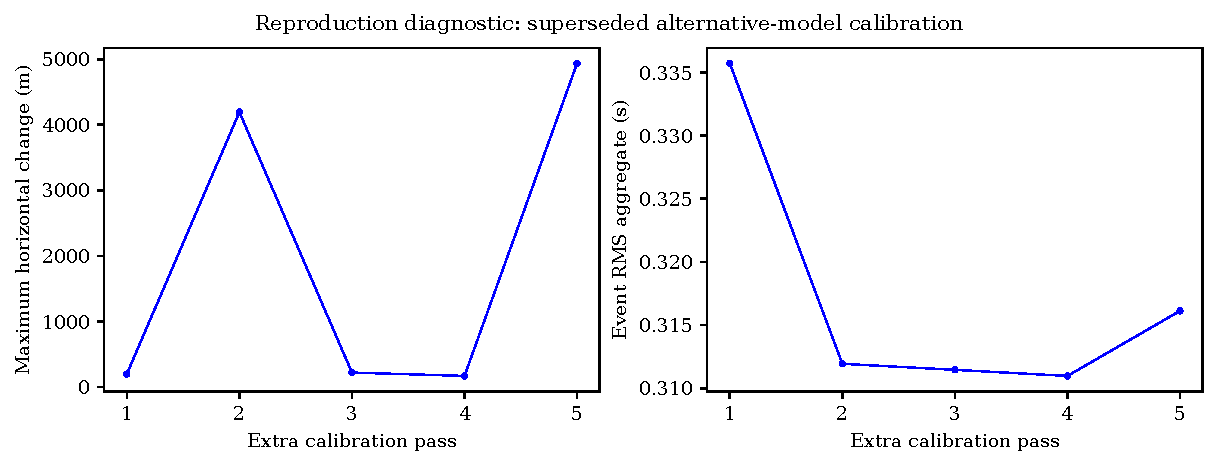
\includegraphics[width=.96\linewidth]{figures/calibration_convergence_diagnostic.pdf}
\caption{Reproduction diagnostic, not a publication figure. Saved convergence trials show kilometer-scale location changes despite similar residual statistics. The model and locations are rejected for scientific interpretation.}
\end{figure}

\paragraph{Observed delays and exploratory HypoDD.}
The 238-event filtered trial supplies 1653 nearest-neighbor pairs and 6362 catalog differential phases. Original response-corrected waveform measurements supply 10,882 channel comparisons, 737 passing channels and 517 coherency-weighted station/phase delays; 13 window failures are retained. The preceding two-second window, 1--15 Hz band and correlation/coherence thresholds are explicit assumptions, not recovered author configuration. Rejected picks or published event solutions are not used to fill gaps.

Generic HypoDD 2.1 was obtained from Waldhauser's official repository at revision \path{fb40407} (full commit in the source receipt). Bounds checks exposed an incorrect output-vector dummy extent in \path{matmult2.f}; it was changed from the column count to the row count, with unchanged multiplication equations. An isolated synthetic matrix assertion checks that fix and never enters empirical data. Source hashes, dimensions, compiler flags and the exact change are recorded in \path{hypodd21_sources.json} and \path{hypodd_build.json} under the follow-up data directory.

Two alternative-profile HypoDD LSQR rounds returned 127 and 126 locations. These are not TomoDD rounds. Six shared phases link clusters; two four-iteration blocks shift weight from catalog to waveform delays, with LSQR damping 50, and a $300^\circ$ gap ceiling. Magnitudes and initial errors set to zero are unused format fields, not measured quantities. LSQR error columns are not interpreted as uncertainties. Quadrants about $14.14^\circ$E, $40.82^\circ$N provide explicit alternative SVD subsets; they do not recreate the paper's four numerical selections. Smaller underconstrained components failed, so only the largest connected component in each quadrant was attempted. NW, SW and SE return 40, 16, 22 estimates; NE diverges and supplies no valid output. The largest conditional 95\% depth errors are 4494.8, 662.9, 507.7 m, respectively. These conditional errors and unstable locations cannot establish the publication's spatial precision. No S7 panel is promoted.

\begin{figure}[H]\centering
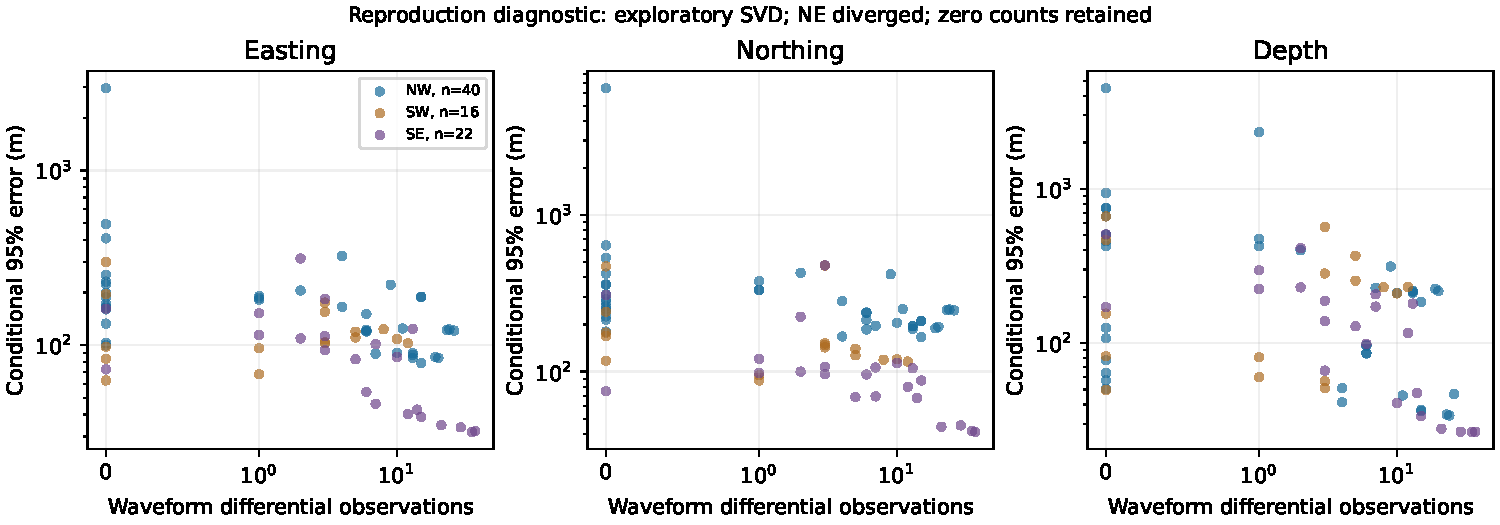
\includegraphics[width=.96\linewidth]{figures/relocation_uncertainty_diagnostic.pdf}
\caption{Reproduction diagnostic, not Figure S7. Conditional SVD errors for three exploratory connected components; the fourth diverged. Zero waveform-difference counts are retained on a symmetric-log abscissa. Error bars cannot validate unreviewed events or the background model.}
\end{figure}

\paragraph{Provenance and remaining prerequisites.}
The authorized De Siena et al. (2017) article cites the original Battaglia model and links PANGAEA 875535. Its inspected metadata list derived locations, attenuation products, geochemistry and map material; no numerical original $V_p/V_s$ grid is identified. Those derived products were not downloaded as analysis inputs. At that checkpoint the model was quarantined. It is now explicitly authorized as a reference input; the new grid-derived results above supersede this historical completion record. Source receipts, URL and hash are recorded; no correspondence was initiated. Exact Cal\`o--Tramelli layer depths and velocities also remain missing, but did not prevent these explicitly alternative trials. TomoDD using the stated fixed 3D background, accepted-location magnitudes, the four specified S7 subsets and their dependent structural panels remain uncompleted. Reviewed phases, stable calibration, verified numerical grid/coordinates/depth convention and regional-averaging masks remain prerequisites. Coverage remains sparse and RAN waveforms credential-gated. Additional observations alone do not resolve the failed calibration.

The complete own-run controls, input serialization, logs and outputs, including failures, are preserved in \path{data/calibration_followup/run_records.zip} with member hashes. Code and commands are in \path{docs/CALIBRATION_FOLLOWUP.md}. The incremental rebuild executes these trials and reports scientific failures separately from successful software execution; it does not claim a full-period reproduction. Earlier magnitude, focal-mechanism and hybrid statuses are unchanged.


\section{Supporting results and validation}
The historical 1,003-association cohort has \CurrentPicks{} merged picks and \CurrentEvents{} provisional associations; the separately numbered expanded cohort is described above. Probability bounds, S-pick exclusions, the six-pick minimum, unique assignment and valid pick indices are checked. Synthetic homogeneous-medium, analytic and injected-signal fixtures are isolated under \path{tests/results}. They test software assertions only and are excluded from empirical catalogs, magnitude measurements and paper figures. Earlier rebuilds ran the equation and layered-ray checks; their retained pass records are not observations. The current grid rebuild executes the distinct validation described below.

The present S--P check includes \CurrentSPPairs{} paired observations, of which \CurrentBadSP{} are nonpositive. There are \CurrentCPOZ{} associated CPOZ P arrivals. These defects and the alternative velocity profile prevent treating raw associations as validated locations. Internal residuals from the same model do not establish absolute accuracy. The location-check tables retain failed observations. The previous generic/retrained comparison on an unlabeled 1600 s CMIS window produced 17 P/4 S and 11 P/55 S picks respectively; the 120 s CSOB window produced zero and one pick. Those counts remain supporting evidence only, not training or labeled-accuracy reproduction, and are not inserted in S4. An analytic vertical-ray check of the published alternative gives maximum P/S errors of 0.040642/0.072342 s on the 0.1 km eikonal grid; halving the spacing reduces them to 0.020321/0.036171 s. This confirms first-order interface discretization behavior, not the physical accuracy of the alternative profile. The numerical checks and refinement results are saved in \path{tests/results/profile_ray_checks.csv}.

The continuation adds \path{scripts/association_quality.py}, which flags nonpositive travel times, nonpositive S--P, S-only associations and depth-boundary solutions without changing the provisional event list. The first two flags exclude an event from magnitude equations, calibration anchors and the VELEST precision experiment because they violate arrival causality. This explicit necessary screen does not reproduce the paper's manual false-event review. Five baseline multi-station waveform examples were inspected: a strongly recorded event supports functioning detection, while other examples contain late coda picks, arrivals before the fitted origin or unclear onsets. The selection was diagnostic rather than random; it supplies no precision or recall estimate. The original arrays, plotted review and qualitative notes are retained in \path{data/resumption/baseline_association_review}. None of the baseline's 53 provisional magnitudes belonged to the 102 events failing causality. All five updated diagnostic pages were also inspected after the corrected association. They include clearly recorded events, late or coda-associated phase marks, and a real-looking signal whose fit reaches the lower depth bound. Passing causality therefore cannot validate depth or phase identification. Current observations and hashes are recorded in \path{data/resumption/current_association_visual_review.json}; no manual phase edits or event acceptance were inferred from this small diagnostic sample.

The new S4A calculation uses original CSOB waveforms starting at 20 May 2024 20:10:03 UTC, exactly two hours after the event time in the official INGV bulletin. This is a literal interpretation of the caption, not an extracted figure coordinate or an asserted exact match. The bulletin provides contextual timing only; these example picks do not seed the catalog. The trained artifacts and their hashes are in \path{data/continuation/benchmark_window.json}. No labels, predictions or training records from Tan's outputs are used. The released repository's file listing contains trained weights, workflow code and derived products, but no trace-level training labels, split or augmentation manifest. Only the file listing was inspected; prohibited code and output contents were not read. The archived R61 release (Zenodo 16562216, version 1.0) was also directory-listed using HTTP byte ranges. Its permitted trained weights and model configuration were decoded and are byte-identical to the current method artifacts. The archive lists no original training waveform/label, split or augmentation files. Its separately listed association-pick table was not retrieved. The directory, ranges and hashes are recorded in \path{docs/zenodo_release_inventory.json}.

For preliminary differential times, ten nearest neighbors are selected from causally consistent, nonboundary provisional locations. P uses Z; S uses N and E separately. Original observations are response-corrected to velocity, filtered from 1--15 Hz, and cut from $-0.25$ to $+1.75$ s around each own pick. An integer correlation lag within $\pm0.25$ s precedes a cross-spectral phase-slope correction. With angular frequency $\omega$, cross spectrum $S_{xy}$ and magnitude-squared coherence $\gamma^2$, the correction minimizes $\sum_f w_f[-\arg S_{xy}-\omega\delta]^2$, where $w_f=\gamma^2/(1-\gamma^2)$ with a $10^{-6}$ denominator floor. Welch spectra use 64-sample Hann segments and 32-sample overlap. Correlation and mean coherence must each exceed 0.6; boundary lags and residual corrections above one sample are flagged. These explicit settings are assumptions where Tan's written description is incomplete, not recovered author settings. The differential travel time is $(p_a-o_a)-(p_b-o_b)-\delta_{b-a}$, in seconds. Saved observations, measurements and failures are in \path{data/continuation/differential_waveform_windows.npz}, \path{data/continuation/differential_times.csv} and \path{data/continuation/differential_time_failures.csv}. Synthetic zero-lag, known-delay and reversal tests remain isolated under \path{tests/results}. No inferred relocation precision or accepted event coordinates follow from this pilot.

The earlier 1,003-association checkpoint measured \CurrentAmplitudes{} channel amplitudes, with \CurrentSNR{} passing SNR and \CurrentMagnitudeEdges{} accepted difference equations. It returned \CurrentMagnitudes{} provisional magnitudes. These historical outputs are retained for comparison with the distinct current-grid cohort; they no longer supply Figure S8. Candidate measurement errors and quality failures are retained in the JSON/CSV records. The old 140-measurement, 23-SNR, zero-edge result is superseded for the current sample and preserved in Git and the quarantine audit trail.

\subsection*{Additional observational checks}
The CPOZ diagnostic contains 64 P-aligned observed waveforms. It does not implement the relocated ring-sector test.

Spectral measurements were calculated for 822 of 822 template crossings. None is confirmed as a hybrid event; spectral windows use correlation alignment and still require onset/coda review.

Catalog frequency-index screening measured 20631 station windows for 908 provisional events. Station FIs are averaged; no low-frequency candidate is classified as a confirmed hybrid without onset and coda review.

The alternative-profile VELEST experiment used 120 provisional events. Both real precisions were attempted with identical serialized inputs.

Maximum 32/64-bit differences were 0.000 km/s for Vp and 0.000 km/s for Vs, with 0.000 km in fitted depth.

Both runs pass the necessary positive-Vp-greater-than-Vs check. This ordering and numerical agreement do not replace reviewed phases or the documented regional calibration; no experimental fit is accepted for S6 or relocation.

The 32-bit experiment has event-RMS aggregate 0.389 s.

The 64-bit experiment has event-RMS aggregate 0.389 s.


\subsection*{Review of low-frequency candidates}
The additional low-frequency review is recorded in \path{data/resumption/catalog_frequency_visual_review.json}, with numerical windows and their source/hash index in \path{data/continuation/catalog_frequency_review.npz} and \path{data/continuation/catalog_frequency_review_index.json}. The diagnostic selects the two highest station SNRs and the lowest station FI per candidate, retaining distinct stations. It displays original response-corrected Z observations from $-20$ to $+16$ s, with longer processing context and a separate 0.2--6 Hz curve. FI and SNR labels refer to the previously saved measurement windows, not a recomputation from the display. Dotted markers show other provisional arrivals; they are not validated coda labels. No qualitative review note is used to alter the catalog, and the station measurements' reviewed-onset flags remain false. The diagnostic PDF is retained in the repository and excluded from the paper and figure-comparison deliverable.

\subsection*{Magnitude statistics and comparison boundary}
The conditional magnitude-frequency fit gives $M_c=0.4$ and $b=1.01 \pm 0.19$ from only 21 selected magnitudes at or above the pilot completeness level. The quoted Shi--Bolt standard error excludes coverage, selection and magnitude-calibration biases. This calculation does not establish population completeness or a regional b-value.


No Tan-derived result-table statistics are used in this paper. The comparison PDF contains only clearly labeled published figure references and the eligible independent counterparts.

\section{Authorized-grid calibration and fixed-grid relocation}
This section supersedes the calibration completion statements in earlier checkpoints. Earlier experiments are retained separately as historical diagnostics. The present run uses the expanded cohort; integer event identifiers must not be joined to the older 1,003-event cohort.

\paragraph{Reference input and transformation.}
Tan et al.'s distribution at revision \path{f84c9c9d} (full revision in the source receipt) supplies \path{models/3d_vmod}, attributed to Battaglia et al. (2008; doi:10.1111/j.1365-2478.2007.00687.x). The current instruction explicitly permits that file as a starting/reference input. Its unchanged 122,853-byte copy is \path{data/grid_calibration/reference_grid.original}; SHA-256 is \path{dc36fe2a542fc7a3b6c473c48ec109c53ddd77a1721f509b920fea97fb0166f3}. It is not claimed to be an independently retrieved original 2008 array. The grid contains 23 longitude, 14 latitude and 27 depth nodes, ordered longitude fastest, then latitude and depth. Longitude/latitude are degrees east/north, depth is km below sea level, $V_p$ is km/s, and the second volume is dimensionless $V_p/V_s$. Pointwise $V_s=V_p/(V_p/V_s)$. Depth extends from $-0.5$ to a 200 km padding node; the shallow model ends at 7 km. The original article describes an 18 by 18 by 9 km volume with 0.5 km spacing, unlike these irregular/padded axes. The historical transformation remains undocumented. The generic TomoDD reader and manual establish the encoding; the current 3D file is not regridded.

Regional averaging uses explicit assumed boxes: $14.01$--$14.21^\circ$E, $40.76$--$40.87^\circ$N for the caldera and $14.11$--$14.16^\circ$E, $40.80$--$40.84^\circ$N for Pozzuoli--Solfatara. Node weights are $\cos(\mathrm{latitude})$; $V_p$ and pointwise $V_s$ are averaged separately. Exact $V_p=0.1$ km/s nodes are interpreted as nonsolid/air and excluded from the 1D average. The first entirely solid plane, 0.1 km deep, extends upward to $-0.5$ km. Horizontal padding and the terminal 200 km layer are excluded from regional depth integration. These masks, layer boundaries and weights are assumptions where Tan gives region names without numerical masks. They do not recover an undocumented transformation.

\paragraph{Independent observations and corrections to the failed pilot.}
The saved expanded input contains 868 processed files, 26 station names and 8511.520 union channel-hours. Independent association times span 2022-01-21T01:14:48.080 to 2025-03-20T23:58:58.807, with large gaps; this is not full-period coverage. 916 of 1015 associations have positive travel times and no observed nonpositive S--P pairs. Calibration additionally requires at least four P and two S picks, more than ten total picks, gap below $180^\circ$ and no initial 0/8 km depth-bound hit, leaving 38 unreviewed candidates. This is not Tan's manually selected 373-event sample. No routine catalog or author result selects these events.

The first eight-layer attempts produce $V_p\leq V_s$ after the station-delay inversion and are rejected. The generic VELEST guide recommends avoiding low-velocity layers initially, locating events before velocity inversion, merging similar unresolved layers and damping unresolved deep velocities. Accordingly LOWVELOCLAY is zero, prelocation uses 14 iterations, and four layer tops are $-0.5,1,3,5$ km. The deepest velocity damping is 100, other layer damping is 1; deeper unconstrained velocities are not freely fitted. A failed damping-1000 attempt overflowed the fixed-width output field and is retained as a serialization failure. The corrected four-layer run preserves physical ordering. It performs two seven-iteration calibration rounds followed by three declared convergence checks, without changing observations or relaxing the paper's final filters. The reference P delay is fixed at IV.CFB3.. The last-pass model, not the still-moving second-round fit, supplies the catalog run.

\paragraph{Validation and catalog filtering.}
Both regional fits satisfy the stated local stability gates: every horizontal/depth change below 100 m, velocity change below 0.05 km/s, and station-delay change below 0.02 s in the final extra pass. The lower converged unweighted phase RMS is 0.218 s (caldera). These are numerical gates, not absolute accuracy. Regional starts still give maximum differences of 654.7 m horizontally and 1.04 km in depth. Complete 32/64-bit paths differ by 557.8 m horizontally, 0.89 km in depth, 0.32 km/s in velocity and 0.25 s in station delay. Starting both precisions from the same converged fit instead gives identical printed coordinates and velocities. Thus a small final change does not remove path sensitivity; printed equality does not bound unprinted differences. Reviewed phases and independent absolute-location validation remain undone; held-out refitting is reported in the additional validation section. The fit is not accepted as a scientific catalog.

All 916 usable events enter the fixed-model run. Three passes precede $|r|>0.4$ s rejection; another pass precedes $|r|>0.3$ s rejection. The fifth pass and final six-pick, 0.25 s reported-RMS and $300^\circ$ gap filters leave 216 exploratory locations. Fixed models and station corrections were checked after each pass; rejected phases are not replaced. The generic reported event statistic differs from unweighted phase RMS, as verified in the preceding checkpoint.

\paragraph{Observed differential times and TomoDD.}
round 1: 132 outputs, 124 gap passes; round 2: 124 outputs, 123 gap passes. both fixed-grid rounds executed; validation pending. The neighbor graph and windows belong to this expanded event set; no old-cohort waveform cache is reused. Exact measured counts, failed windows, controls and residuals are in \path{data/grid_calibration/merged4/tomodd}. Original absolute picks supply phase-pair times; response-corrected two-second windows supply coherency-weighted delays. Ten nearest neighbors, 1--15 Hz filtering, correlation/coherence at least 0.6, maximum lag 0.25 s, six-phase clustering links, LSQR damping 50 and two four-iteration weight blocks are explicit assumptions where configuration is unpublished. JOINT=0 fixes the 3D grid. A second round rebases travel-time differences to the independently updated origins. Generic method tables required by the solver are separated from the example observations in its distribution. No author-fitted corrections, velocity model or earthquake result is substituted. Available provisional numerical results now populate Figures 2--3, S6--S7, S10--S13; scientific acceptance remains unresolved.

\paragraph{Display verification and scientific boundaries.}
Every current generated figure is rebuilt from saved numerical products by \path{scripts/publication_plots.py}. Input/output hashes and panel correspondence are in \path{data/grid_calibration/style/plot_inventory.json}. Figure S5 uses the printed 0--5 km depth limits and ticks 0,1,2,3,4,5; Figure 1A has printed ticks 0,2,4 but unlabeled endpoints, so 0--5 km is an explicitly approximate normalization rather than an exact recovery. Neither numerical table changes. Magenta denotes depths above 5 km: 4 in 1A and 2 in S5; white is reserved below zero. Missing magnitudes remain crosses. The area law $0.7+3\,10^{M_d-2}$ points squared is a display assumption, not a recovered published formula. S4/S15 do not print a numerical spectral color scale; their disclosed normalized-PSD display is $-80$ to 0 dB, with white/black under/over colors. Counts and ranges are saved in \path{spectral_scales.json}. S2 uses documented instrument classes; no copied relief or elevation colorbar is manufactured. Diagnostic figures have consistent typography but are explicitly not publication figures. Figure 3 now has an explicitly provisional counterpart. Figure 4A--B still lack a returned mechanism; no beachball is invented.

\paragraph{Rebuild and audit trail.}
Run \path{.venv/bin/python scripts/rebuild_grid_workflow.py} from the repository root. It checks the existing independent processing checkpoint, rebuilds generic solvers, regenerates grid-derived starts, executes calibration/validation and both relocation attempts where supported, plots saved data and compiles both PDFs. The saved independent waveform-window cache may be reused only with matching input/output hashes; \path{--remeasure} recomputes it from recordings. The current procedure does not imply that unfinished full-period acquisition or inference was executed. Controls, own serialized inputs, logs and results are preserved in \path{data/grid_calibration/run_records.zip}; machine-readable procedure and scientific outcomes are separate. Earlier models/results remain in Git and their labeled historical directories. The current grid authorization changes input eligibility, not numerical validation requirements.
The generic solver originally overwrote earlier clusters' residual tables. The output-only patch appends every cluster; final gaps now use only stations with positive-weight retained residuals. This correction changes the trial gap-passing counts and supersedes the last-cluster-only diagnostics, which are preserved separately. All 124 final output events have residuals represented. The final per-observation RMS is 0.0430 s for waveform differences and 0.1086 s for picked-phase constraints. Neither value establishes correct event identity or absolute location accuracy.

\begin{figure}[H]\centering
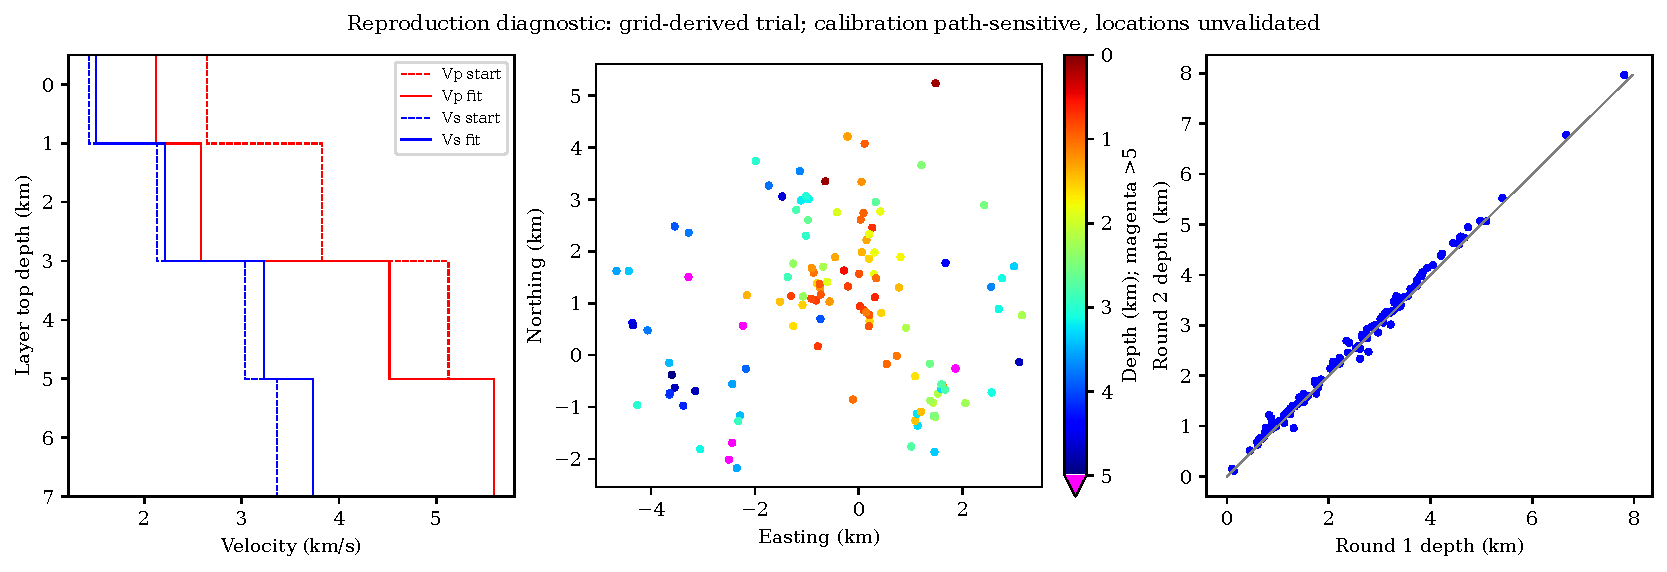
\includegraphics[width=.97\linewidth]{figures/grid_calibration_diagnostic.pdf}
\caption{Reproduction diagnostic, not a publication panel. Grid-derived starting and independently fitted layer velocities, exploratory second-round TomoDD locations and the change in depth between rounds. Fixed color limits are 0--5 km; magenta retains deeper results. Calibration path dependence and unreviewed phases prevent interpreting these patterns as recovered faults.}
\end{figure}

\section{Additional validation and provisional analyses}
The new figures expose available numerical results rather than replacing unvalidated locations with blank panels. Independent generation does not establish their scientific accuracy. The frozen calibration cohort and original 3D grid are unchanged; the retained original grid hash and conventions are documented above.

\paragraph{Precision and convergence diagnosis.}
The original 32/64-bit initial model, station file, observations and control files are byte-identical. Both prelocation runs stop at 14 iterations. Their maximum depth difference is initially 0.02 km and grows to 0.89 km through coupled updates. Common-start tests give identical printed round-1 locations and zero printed round-2 depth difference; the latter horizontal difference is 11.1 m. The small final update can result from four-backup stagnation and is not proof of an optimum. Backup decisions diverge in round 2; subsequent paths stop either at iteration limits or after four backups. Instrumented, otherwise unchanged generic solvers reproduce the original output bytes. The damped prelocation normal-matrix condition numbers range from 2372 to 3313; this test does not support a catastrophic linear-solve failure. Nonlinear paths, ray changes and two-decimal restart serialization amplify initial differences. Exact arithmetic attribution of every ray transition remains untested.

Repeated fixed-model prelocation, up to ten 14-iteration passes in each precision, still fails the unchanged 100 m stability gate. The 64-bit last pass moves an event 282 m horizontally and 0.24 km vertically. More iterations alone do not resolve this oscillation. No locations from this failed correction are substituted. Every fifth calibration event was withheld: 30 events train the model, 8 events (126 phases) test it. Unweighted held-out phase RMS is 0.2177 s for the starting profile and 0.2198 s for the refitted profile. A smaller solver event statistic is a different quantity and cannot reverse this failed prediction check. Manual phase/association review and absolute-location validation remain necessary. The own fitted 1--3 km layer has Vp/Vs=1.17. Passing positive-velocity ordering alone does not establish a plausible or well-constrained elastic structure; this low ratio warrants scientific review.

\paragraph{Relocation and conditional uncertainty.}
Across 124 common events, rounds 1 and 2 differ by a median 113.3 m and maximum 384.0 m horizontally; median absolute depth change is 0.095 km and maximum 0.382 km. On the same 399 waveform constraints, RMS improves from 0.0414 to 0.0400 s. The same 4395 picked-phase constraints improve from 0.1084 to 0.1020 s. Fixed grid, positive travel times, all-cluster residual coverage and recomputed station-gap checks pass. These are internal checks, not absolute accuracy. 34 events have no retained waveform correlations. No event passes S9's $NCCP+NCCS>100$ filter.

SVD was attempted on every connected component with at least four events in four explicit quadrants; 90 estimates were returned. Their 2-sigma depth errors reach 4.002 km, whereas the publication describes most coordinate errors near 10 m. The regional masks, sample sizes and starting locations differ, so this is a consequential failure to recover comparable precision, not a contradiction of the original estimates. S7 retains the large uncertainties. S12 uses 118 recorded component traces joined to the same relocated cohort. Sector masks and spectral normalization are explicit assumptions; no published depth bands select our events.

\paragraph{Magnitude and source mechanisms.}
The relocated-subset magnitude stage measured 5929 channels, with 1626 passing 5 dB, and inverted 884 relative-amplitude equations to obtain 65 magnitudes. Routine duration magnitudes enter only as regularization after independent detection and location. All accepted components have full numerical rank; formal errors are conditional on the response, location, weighting and unit regularization assumptions. Maximum curvature gives $M_c\simeq 0.0$ and the conditional likelihood estimate is $b=0.866\pm 0.110$ (41 above $M_c$). This selected, discontinuously observed sample cannot establish the published full-catalog $M_c=0.4$ or $b=0.97$.

SKHASH 1.1.5 now executes on 76 automated measurements from 8 events; 35 pass an explicit sign/SNR screen. Seven events fail the minimum-eight-polarity rule, and event 641 fails the unchanged azimuthal-gap rule (186.158 versus 90 degrees). No mechanism is returned. These are unreviewed candidate polarities, not Tan's manual measurements; no supplied mechanism or S/P value is used. Independent gCAP/FK processing, reviewed S/P measurements and event-specific waveform settings remain incomplete. The generic software is isolated in \path{.venv-skhash} because its NumPy requirement differs from the main analysis environment; the main NumPy 2.4.6 was restored. Dependency caches remain under the existing user pip cache; scientific products remain inside this repository.

\paragraph{Commands and evidence.}\begingroup\small\raggedright
\path{scripts/diagnose_grid_paths.py}, \path{scripts/settle_grid_prelocation.py}, \path{scripts/grid_uncertainty.py}, \path{scripts/downstream_checks.py --dataset grid}, \path{scripts/grid_focal_attempt.py} and \path{scripts/grid_panel_data.py} generate the new saved products. The single procedure \path{.venv/bin/python scripts/rebuild_provisional_workflow.py} executes these stages and compiles both documents. \path{docs/PROVISIONAL_CONTINUATION.md} records the full command and input chain, including acquisition scope. Procedure completion is separate from scientific acceptance.
\par\endgroup

\section{Additional observed coverage and independent calibration trial}
The latest separately frozen extension contains 997 observed files from 26 station names, 8706.970 union channel-hours, 134,483 picks and 1,023 provisional associations (7,410 assigned picks). All returned study-period files in its manifest were processed. Instrument sensitivity and response stages cover all 8706.970 measured channel-hours; this checks epoch coverage, not absolute instrument calibration. The source-level gaps and failed/pending requests remain in its station-by-time ledger. Full-period acquisition remains unfinished, not demonstrated inaccessible. RAN waveform credentials remain unavailable.

The same grid-derived inversion and relocation procedure was attempted on this cohort. S6: 219 provisional events; 3: 123 provisional events; independently rerun downstream stages return 80 conditional SVD estimates, 67 amplitude magnitudes, 0 mechanisms, and 383 S-P pairs. Failed computational stage: None: all requested solver stages executed; scientific acceptance remains false. No prior cohort event ID is reused as a solution. The additional numerical views are explicitly provisional; the 90 SVD estimates, 65 magnitudes and CPOZ gathers elsewhere retain the frozen 1,015-association cohort. These counts must not be combined as separate earthquakes.

Unchanged daily association inputs reuse this implementation's own recorded solve only after checking the complete original checkpoint, station data, settings and exact multiset of numerical pick inputs. Identical-time row order and overlapping-file aliases can differ; indices are explicitly remapped to current original observations. Changed days run GaMMA again. This is not a claim that a new solve with another row ordering would be bitwise identical. A redundant association pass was interrupted and is not counted as complete.

\begingroup\small\raggedright Evidence and commands: \path{data/coverage_extension/processing_checkpoint.json}, \path{association_reuse.json}, \path{station_coverage.csv}, \path{unobserved_channel_intervals.csv}, \path{request_ledger.csv.gz} and \path{calibration/execution.json}, all under \path{data/coverage_extension/}. Run \path{scripts/freeze_coverage_extension.py} for the source ledger, \path{scripts/calibrate_coverage_extension.py} for the independent trial, and \path{scripts/publication_plots.py} for its saved numerical counterparts. Full executed solver controls and logs are preserved in \path{data/coverage_extension/calibration/run_records.zip}.
\par\endgroup

The extended-cohort full-path precision difference remains 0.89 km in depth. Its 38-event calibration input multisets and controls match the earlier trial, with tied-phase ordering recorded explicitly; extra coverage therefore did not add calibration leverage. Between TomoDD rounds, maximum horizontal and depth shifts are 386.2 m and 0.372 km. Conditional SVD depth errors reach 1.337 km. Their changed subset size is not proof of better absolute accuracy. Conditional magnitude statistics are Mc=0.0, b=0.866 +/- 0.110; they remain selected-subset descriptions, not population completeness.


\section{Limitations and unfinished analyses}
No publication panel is fully independently reproduced. 53 panel/views have partial numerical counterparts; 10 are unreproduced. Independent calculation and scientific agreement are assessed separately.
 Routine-context permissions and the 2025 displacement gap are resolved. The full continuous download/processing workload remains unfinished. Exact Cal\`o--Tramelli layer values are an external-input limitation; the distributed fixed 3D artifact is now authorized, while its original transformation remains unresolved and the new calibration remains path-sensitive. RAN credentials are a specific access limitation.

Accepted calibrated locations, reliable multiyear magnitudes/completeness, human-reviewed polarities and S/P ratios, accepted SKHASH/gCAP mechanisms, exact original regional masks, manual deep-event validation and three-year hybrid clustering remain incomplete. This continuation generated FK Green functions and provisional gCAP fits; these stages are no longer described as unrun. The per-candidate table and frequency-band validation explain why no mechanism is accepted. Training labels/splits and some inversion settings remain incompletely specified. Author-derived results are not substituted for these missing or unaccepted analyses.

\section{Figure-by-figure record}
The machine-readable \path{docs/panel_record.json} records every panel's written specification, parameters, exact input paths, executed data/plot commands, saved products and limitation. The raw-waveform manifest is \path{docs/continuation_processed_inputs.json}; its intervals are a frozen checkpoint, not the full queue. Context data use \path{continue_context.py}; all current displays use \path{scripts/publication_plots.py}. S1 displays the expanded processing coverage. S2 is audited by \path{scripts/station_geometry.py}; S15C retains its original-waveform recipe. Panels with no usable numerical result have explicit missing-result notices. Available provisional results and clearly labeled alternative examples are plotted rather than withheld for failing validation.
\begingroup\footnotesize\begin{longtable}{>{\raggedright\arraybackslash}p{.12\linewidth}>{\raggedright\arraybackslash}p{.25\linewidth}>{\raggedright\arraybackslash}p{.52\linewidth}}
\toprule Panel/view & Quantity & Status, specification and limitation\\\midrule\endhead
1A & INGV event map and large-event markers & partially reproduced. Main p.71, Fig.1 caption. 2005-01-01 to 2025-03-20; origin 14.14 E, 40.82 N; sea-level depth; Md$>$=4 markers Display: depth-colored jet\_r circles, area=0.7+3*10**(Md-2) points squared; missing Md shown as crosses. Exact publication area law unspecified. Full color ranges: 0--8 km for 1A, 0--6 km for S5. Display bounds and off-view counts saved in routine\_plot\_scope.csv.. Current catalog snapshot differs from the historical snapshot: 12,503 located study events versus 12,083. No tuning to published counts. Natural Earth coastline is a display substitute; the original relief/inland-zero contour has not been reconstructed.\\[3pt]
1B & Vertical displacement at Pozzuoli port & partially reproduced. Main p.71, Fig.1 caption. 128 historical entries: 114 leveling surveys, 13 source-provided estimates and one source-provided graphical reconstruction. Source classes preserved separately. Daily GNSS 2000-05-29 through 2025-03-20; median datum from 23 overlapping leveling epochs, +/-15 days. Month-only dates placed on day 15 for display.. Benchmark equivalence and datum-joining convention are assumed because the exact original stitching recipe is not specified. Calendar gaps remain unfilled; no missing recent-data blocker through 2025-03-20.\\[3pt]
1C & Temporal seismicity and cumulative counts & partially reproduced. Main p.71, Fig.1 caption. 2005-2025; cumulative Md$>$0.2; study interval 2022-01-21 to 2025-03-20. Monthly counts and exact-time cumulative Md$>$0.2 reconstructed from the current routine snapshot; historical count differences unresolved. March 2025 is a partial month.\\[3pt]
2A & Catalog seismicity rates by region & not reproduced. Main p.72, Fig.2 caption. Central vs ring/other regions; 54319 vs 12083 catalog events; time bin unspecified. Grid input explicitly authorized; historical transformation and averaging masks not recovered exactly. Local calibration convergence passes, full-path precision and start-model dependence do not. Unreviewed phases and sparse coverage; no accepted relocated scientific catalog. both fixed-grid rounds executed; validation pending\\[3pt]
2B & Depth versus time, symbol size by magnitude & not reproduced. Main p.72, Fig.2 caption. Sea-level depth; near-surface 0-0.5 km; central 0.5-2.1; ring sectors to 3.7 km. Grid input explicitly authorized; historical transformation and averaging masks not recovered exactly. Local calibration convergence passes, full-path precision and start-model dependence do not. Unreviewed phases and sparse coverage; no accepted relocated scientific catalog. both fixed-grid rounds executed; validation pending\\[3pt]
3/\allowbreak{}map & Epicentral spatial pattern & not reproduced. Main p.73, Fig.3 caption. Relative origin 14.14 E, 40.82 N; sea-level depths. Grid input explicitly authorized; historical transformation and averaging masks not recovered exactly. Local calibration convergence passes, full-path precision and start-model dependence do not. Unreviewed phases and sparse coverage; no accepted relocated scientific catalog. both fixed-grid rounds executed; validation pending\\[3pt]
3/\allowbreak{}northing-depth & Depth versus northing & not reproduced. Main p.73, Fig.3 caption. Relative origin 14.14 E, 40.82 N; sea-level depths. Grid input explicitly authorized; historical transformation and averaging masks not recovered exactly. Local calibration convergence passes, full-path precision and start-model dependence do not. Unreviewed phases and sparse coverage; no accepted relocated scientific catalog. both fixed-grid rounds executed; validation pending\\[3pt]
3/\allowbreak{}easting-depth & Depth versus easting & not reproduced. Main p.73, Fig.3 caption. Relative origin 14.14 E, 40.82 N; sea-level depths. Grid input explicitly authorized; historical transformation and averaging masks not recovered exactly. Local calibration convergence passes, full-path precision and start-model dependence do not. Unreviewed phases and sparse coverage; no accepted relocated scientific catalog. both fixed-grid rounds executed; validation pending\\[3pt]
4A & Ring-sector focal mechanisms and seismicity & not reproduced. Main p.74, Fig.4; supplement S6-S7. High quality: SKHASH A or Kagan angle$<$30 deg; gCAP preference with stated exception. Grid input explicitly authorized; historical transformation and averaging masks not recovered exactly. Local calibration convergence passes, full-path precision and start-model dependence do not. Unreviewed phases and sparse coverage; no accepted relocated scientific catalog. both fixed-grid rounds executed; validation pending\\[3pt]
4B & Central/onshore focal mechanisms and seismicity & not reproduced. Main p.74, Fig.4; supplement S6-S7. High quality: SKHASH A or Kagan angle$<$30 deg; gCAP preference with stated exception. Grid input explicitly authorized; historical transformation and averaging masks not recovered exactly. Local calibration convergence passes, full-path precision and start-model dependence do not. Unreviewed phases and sparse coverage; no accepted relocated scientific catalog. both fixed-grid rounds executed; validation pending\\[3pt]
S1 & Station data-availability timeline & partially reproduced. Supplement S12 caption; S2 methods. 48 stations; continuous-data availability. Expanded processed subset: 868 files, 8511.520 channel-hours; full-period queue remains unfinished. No requested-but-failed interval is counted.\\[3pt]
S2 & Station map & partially reproduced. Supplement S13 caption; S2 methods. 23 broadband, 9 short-period, 16 accelerometers. The published 48-instrument membership is not verified. Two released-coordinate pairs coincide; no deployment alias mapping justifies collapsing or removing identifiers.\\[3pt]
S3A & Noise example: waveform, phase labels, spectrogram & not reproduced. Supplement S14 caption; S2-S3. 30-s windows; P/S labels; D amplitude rescaling. Exact training traces and labels not identified from permissible metadata. Retraining was not repeated; permitted trained weights used for inference only.\\[3pt]
S3B & Single-event example: waveform, phase labels, spectrogram & not reproduced. Supplement S14 caption; S2-S3. 30-s windows; P/S labels; D amplitude rescaling. Exact training traces and labels not identified from permissible metadata. Retraining was not repeated; permitted trained weights used for inference only.\\[3pt]
S3C & Two overlapping events: waveform, phase labels, spectrogram & not reproduced. Supplement S14 caption; S2-S3. 30-s windows; P/S labels; D amplitude rescaling. Exact training traces and labels not identified from permissible metadata. Retraining was not repeated; permitted trained weights used for inference only.\\[3pt]
S3D & Five overlapping copies of one event: waveform, phase labels, spectrogram & not reproduced. Supplement S14 caption; S2-S3. 30-s windows; P/S labels; D amplitude rescaling. Exact training traces and labels not identified from permissible metadata. Retraining was not repeated; permitted trained weights used for inference only.\\[3pt]
S4A & Swarms at CSOB: waveform, spectrogram, original and retrained picker scores & partially reproduced. Supplement S15 caption; S2-S3. 120 s CSOB window at 2024-05-20 20:10:03 UTC, interpreting the caption two-hour offset literally; 1 Hz highpass, released model settings, thresholds 0.3.. Exact published start is not specified in the caption; no reference phase labels. Different pick counts do not establish accuracy or successful retraining.\\[3pt]
S4B & CMIS noise: waveform, spectrogram, original and retrained picker scores & not reproduced. Supplement S15 caption; S2-S3. 1600 s; coastal noise; phase threshold 0.3. Original and retrained models both executed on independently selected CSOB/CMIS calendar windows. Exact published windows and independent reference annotations remain unidentified; these diagnostics are not the published benchmark.\\[3pt]
S5/\allowbreak{}map & Routine-catalog spatial views; map & partially reproduced. Supplement S16 caption. 12083 events; 1D model and HYPO71 Display: depth-colored jet\_r circles, area=0.7+3*10**(Md-2) points squared; missing Md shown as crosses. Exact publication area law unspecified. Full color ranges: 0--8 km for 1A, 0--6 km for S5. Display bounds and off-view counts saved in routine\_plot\_scope.csv.. Current catalog snapshot differs from the historical snapshot: 12,503 located study events versus 12,083. No tuning to published counts. Natural Earth coastline is a display substitute; the original relief/inland-zero contour has not been reconstructed.\\[3pt]
S5/\allowbreak{}northing-depth & Routine-catalog spatial views; northing-depth & partially reproduced. Supplement S16 caption. 12083 events; 1D model and HYPO71 Display: depth-colored jet\_r circles, area=0.7+3*10**(Md-2) points squared; missing Md shown as crosses. Exact publication area law unspecified. Full color ranges: 0--8 km for 1A, 0--6 km for S5. Display bounds and off-view counts saved in routine\_plot\_scope.csv.. Current catalog snapshot differs from the historical snapshot: 12,503 located study events versus 12,083. No tuning to published counts. Natural Earth coastline is a display substitute; the original relief/inland-zero contour has not been reconstructed.\\[3pt]
S5/\allowbreak{}easting-depth & Routine-catalog spatial views; easting-depth & partially reproduced. Supplement S16 caption. 12083 events; 1D model and HYPO71 Display: depth-colored jet\_r circles, area=0.7+3*10**(Md-2) points squared; missing Md shown as crosses. Exact publication area law unspecified. Full color ranges: 0--8 km for 1A, 0--6 km for S5. Display bounds and off-view counts saved in routine\_plot\_scope.csv.. Current catalog snapshot differs from the historical snapshot: 12,503 located study events versus 12,083. No tuning to published counts. Natural Earth coastline is a display substitute; the original relief/inland-zero contour has not been reconstructed.\\[3pt]
S6/\allowbreak{}map & Initial-location spatial views; map & not reproduced. Supplement S17 caption. Requires verified fixed 2008 grid, documented regional averages and validated independent VELEST inversions.. Grid input explicitly authorized; historical transformation and averaging masks not recovered exactly. Local calibration convergence passes, full-path precision and start-model dependence do not. Unreviewed phases and sparse coverage; no accepted relocated scientific catalog. both fixed-grid rounds executed; validation pending\\[3pt]
S6/\allowbreak{}northing-depth & Initial-location spatial views; northing-depth & not reproduced. Supplement S17 caption. Requires verified fixed 2008 grid, documented regional averages and validated independent VELEST inversions.. Grid input explicitly authorized; historical transformation and averaging masks not recovered exactly. Local calibration convergence passes, full-path precision and start-model dependence do not. Unreviewed phases and sparse coverage; no accepted relocated scientific catalog. both fixed-grid rounds executed; validation pending\\[3pt]
S6/\allowbreak{}easting-depth & Initial-location spatial views; easting-depth & not reproduced. Supplement S17 caption. Requires verified fixed 2008 grid, documented regional averages and validated independent VELEST inversions.. Grid input explicitly authorized; historical transformation and averaging masks not recovered exactly. Local calibration convergence passes, full-path precision and start-model dependence do not. Unreviewed phases and sparse coverage; no accepted relocated scientific catalog. both fixed-grid rounds executed; validation pending\\[3pt]
S7A/\allowbreak{}map & Cluster locations and 2-sigma errors: map and cross-sectional views; map & not reproduced. Supplement S18 caption; S5 methods. Central174, north165, southwest175, east166; HypoDD SVD; Table S1. Grid input explicitly authorized; historical transformation and averaging masks not recovered exactly. Local calibration convergence passes, full-path precision and start-model dependence do not. Unreviewed phases and sparse coverage; no accepted relocated scientific catalog. both fixed-grid rounds executed; validation pending\\[3pt]
S7A/\allowbreak{}easting-depth & Cluster locations and 2-sigma errors: map and cross-sectional views; easting-depth & not reproduced. Supplement S18 caption; S5 methods. Central174, north165, southwest175, east166; HypoDD SVD; Table S1. Grid input explicitly authorized; historical transformation and averaging masks not recovered exactly. Local calibration convergence passes, full-path precision and start-model dependence do not. Unreviewed phases and sparse coverage; no accepted relocated scientific catalog. both fixed-grid rounds executed; validation pending\\[3pt]
S7B & EX uncertainty versus differential-pick count & not reproduced. Supplement S18 caption. Log-log axes; NCCP+NCCS. Grid input explicitly authorized; historical transformation and averaging masks not recovered exactly. Local calibration convergence passes, full-path precision and start-model dependence do not. Unreviewed phases and sparse coverage; no accepted relocated scientific catalog. both fixed-grid rounds executed; validation pending\\[3pt]
S7D & EY uncertainty versus differential-pick count & not reproduced. Supplement S18 caption. Log-log axes; NCCP+NCCS. Grid input explicitly authorized; historical transformation and averaging masks not recovered exactly. Local calibration convergence passes, full-path precision and start-model dependence do not. Unreviewed phases and sparse coverage; no accepted relocated scientific catalog. both fixed-grid rounds executed; validation pending\\[3pt]
S7F & EZ uncertainty versus differential-pick count & not reproduced. Supplement S18 caption. Log-log axes; NCCP+NCCS. Grid input explicitly authorized; historical transformation and averaging masks not recovered exactly. Local calibration convergence passes, full-path precision and start-model dependence do not. Unreviewed phases and sparse coverage; no accepted relocated scientific catalog. both fixed-grid rounds executed; validation pending\\[3pt]
S7C & EX uncertainty density by cluster & not reproduced. Supplement S18 caption. Kernel density estimate; bandwidth unspecified. Grid input explicitly authorized; historical transformation and averaging masks not recovered exactly. Local calibration convergence passes, full-path precision and start-model dependence do not. Unreviewed phases and sparse coverage; no accepted relocated scientific catalog. both fixed-grid rounds executed; validation pending\\[3pt]
S7E & EY uncertainty density by cluster & not reproduced. Supplement S18 caption. Kernel density estimate; bandwidth unspecified. Grid input explicitly authorized; historical transformation and averaging masks not recovered exactly. Local calibration convergence passes, full-path precision and start-model dependence do not. Unreviewed phases and sparse coverage; no accepted relocated scientific catalog. both fixed-grid rounds executed; validation pending\\[3pt]
S7G & EZ uncertainty density by cluster & not reproduced. Supplement S18 caption. Kernel density estimate; bandwidth unspecified. Grid input explicitly authorized; historical transformation and averaging masks not recovered exactly. Local calibration convergence passes, full-path precision and start-model dependence do not. Unreviewed phases and sparse coverage; no accepted relocated scientific catalog. both fixed-grid rounds executed; validation pending\\[3pt]
S8A & Estimated local versus routine duration magnitude & partially reproduced. Supplement S19 caption; S5-S6 methods. 5 s signal, 2 s preceding noise; SNR $>$=5 dB; all available recorded stations; own picked or predicted P arrivals; $>$=2 shared stations; separation $<$ one fifth of station distance; squared zero-lag correlation weights; Md regularization lambda=1 for unique one-to-one matches within 2 s. Initial locations. B uses 0.1 magnitude bins, maximum-curvature Mc, half-bin-corrected likelihood b and formal Shi-Bolt sampling error; no arbitrary minimum sample cutoff.. 61681 channel measurements, 4705 passing SNR, 1163 relative-amplitude equations, 119 provisional magnitudes. Final relocated locations/full exposure remain missing; routine Md is an allowed regularizer, not independent validation.\\[3pt]
S8B & Magnitude-frequency distribution and fitted b value & partially reproduced. Supplement S19 caption; S6 methods. 5 s signal, 2 s preceding noise; SNR $>$=5 dB; all available recorded stations; own picked or predicted P arrivals; $>$=2 shared stations; separation $<$ one fifth of station distance; squared zero-lag correlation weights; Md regularization lambda=1 for unique one-to-one matches within 2 s. Initial locations. B uses 0.1 magnitude bins, maximum-curvature Mc, half-bin-corrected likelihood b and formal Shi-Bolt sampling error; no arbitrary minimum sample cutoff.. 61681 channel measurements, 4705 passing SNR, 1163 relative-amplitude equations, 119 provisional magnitudes. Final relocated locations/full exposure remain missing; routine Md is an allowed regularizer, not independent validation.\\[3pt]
S9/\allowbreak{}map & Filtered-catalog spatial views and feature labels A-D; map & not reproduced. Supplement S20 caption. 38103 events; NCCP+NCCS threshold 100. Unfinished full-period processing and missing calibrated/relocated catalog. Provisional GaMMA diagnostics use an alternative external profile; they are not this panel. Author-derived results are not substituted.\\[3pt]
S9/\allowbreak{}northing-depth & Filtered-catalog spatial views and feature labels A-D; northing-depth & not reproduced. Supplement S20 caption. 38103 events; NCCP+NCCS threshold 100. Unfinished full-period processing and missing calibrated/relocated catalog. Provisional GaMMA diagnostics use an alternative external profile; they are not this panel. Author-derived results are not substituted.\\[3pt]
S9/\allowbreak{}easting-depth & Filtered-catalog spatial views and feature labels A-D; easting-depth & not reproduced. Supplement S20 caption. 38103 events; NCCP+NCCS threshold 100. Unfinished full-period processing and missing calibrated/relocated catalog. Provisional GaMMA diagnostics use an alternative external profile; they are not this panel. Author-derived results are not substituted.\\[3pt]
S10/\allowbreak{}2022 & Annual seismicity map & not reproduced. Supplement S21 caption. Year 2022. Unfinished full-period processing and missing calibrated/relocated catalog. Provisional GaMMA diagnostics use an alternative external profile; they are not this panel. Author-derived results are not substituted.\\[3pt]
S10/\allowbreak{}2023 & Annual seismicity map & not reproduced. Supplement S21 caption. Year 2023. Unfinished full-period processing and missing calibrated/relocated catalog. Provisional GaMMA diagnostics use an alternative external profile; they are not this panel. Author-derived results are not substituted.\\[3pt]
S10/\allowbreak{}2024 & Annual seismicity map & not reproduced. Supplement S21 caption. Year 2024. Unfinished full-period processing and missing calibrated/relocated catalog. Provisional GaMMA diagnostics use an alternative external profile; they are not this panel. Author-derived results are not substituted.\\[3pt]
S10/\allowbreak{}2025 & Annual seismicity map & not reproduced. Supplement S21 caption. Year 2025 through March20. Unfinished full-period processing and missing calibrated/relocated catalog. Provisional GaMMA diagnostics use an alternative external profile; they are not this panel. Author-derived results are not substituted.\\[3pt]
S11/\allowbreak{}swarm-1 & Map of one of four major swarms & not reproduced. Supplement S22 caption. 2022-2025; exact swarm windows not enumerated in caption. Unfinished full-period processing and missing calibrated/relocated catalog. Provisional GaMMA diagnostics use an alternative external profile; they are not this panel. Author-derived results are not substituted.\\[3pt]
S11/\allowbreak{}swarm-2 & Map of one of four major swarms & not reproduced. Supplement S22 caption. 2022-2025; exact swarm windows not enumerated in caption. Unfinished full-period processing and missing calibrated/relocated catalog. Provisional GaMMA diagnostics use an alternative external profile; they are not this panel. Author-derived results are not substituted.\\[3pt]
S11/\allowbreak{}swarm-3 & Map of one of four major swarms & not reproduced. Supplement S22 caption. 2022-2025; exact swarm windows not enumerated in caption. Unfinished full-period processing and missing calibrated/relocated catalog. Provisional GaMMA diagnostics use an alternative external profile; they are not this panel. Author-derived results are not substituted.\\[3pt]
S11/\allowbreak{}swarm-4 & Map of one of four major swarms & not reproduced. Supplement S22 caption. 2022-2025; exact swarm windows not enumerated in caption. Unfinished full-period processing and missing calibrated/relocated catalog. Provisional GaMMA diagnostics use an alternative external profile; they are not this panel. Author-derived results are not substituted.\\[3pt]
S12A & Ring-sector division & not reproduced. Supplement S23 caption; S8. East, southwest, north; sector boundaries by location/depth. 137 independently associated CPOZ P arrivals now exist. Relocated ring-sector selection and manual depth review remain unfinished; internal S-P checks do not establish location accuracy.\\[3pt]
S12B & Ring-sector division in complementary spatial view & not reproduced. Supplement S23 caption; S8. East, southwest, north; sector boundaries by location/depth. 137 independently associated CPOZ P arrivals now exist. Relocated ring-sector selection and manual depth review remain unfinished; internal S-P checks do not establish location accuracy.\\[3pt]
S12C & Common-receiver gather: east / HHZ & not reproduced. Supplement S23 caption. CPOZ; -1 to +7 s about P; $>$4 Hz; north sector ordered by easting, others northing. 137 independently associated CPOZ P arrivals now exist. Relocated ring-sector selection and manual depth review remain unfinished; internal S-P checks do not establish location accuracy.\\[3pt]
S12D & Common-receiver gather: southwest / HHZ & not reproduced. Supplement S23 caption. CPOZ; -1 to +7 s about P; $>$4 Hz; north sector ordered by easting, others northing. 137 independently associated CPOZ P arrivals now exist. Relocated ring-sector selection and manual depth review remain unfinished; internal S-P checks do not establish location accuracy.\\[3pt]
S12E & Common-receiver gather: north / HHZ & not reproduced. Supplement S23 caption. CPOZ; -1 to +7 s about P; $>$4 Hz; north sector ordered by easting, others northing. 137 independently associated CPOZ P arrivals now exist. Relocated ring-sector selection and manual depth review remain unfinished; internal S-P checks do not establish location accuracy.\\[3pt]
S12F & Common-receiver gather: east / HHN & not reproduced. Supplement S23 caption. CPOZ; -1 to +7 s about P; $>$4 Hz; north sector ordered by easting, others northing. 137 independently associated CPOZ P arrivals now exist. Relocated ring-sector selection and manual depth review remain unfinished; internal S-P checks do not establish location accuracy.\\[3pt]
S12G & Common-receiver gather: southwest / HHN & not reproduced. Supplement S23 caption. CPOZ; -1 to +7 s about P; $>$4 Hz; north sector ordered by easting, others northing. 137 independently associated CPOZ P arrivals now exist. Relocated ring-sector selection and manual depth review remain unfinished; internal S-P checks do not establish location accuracy.\\[3pt]
S12H & Common-receiver gather: north / HHN & not reproduced. Supplement S23 caption. CPOZ; -1 to +7 s about P; $>$4 Hz; north sector ordered by easting, others northing. 137 independently associated CPOZ P arrivals now exist. Relocated ring-sector selection and manual depth review remain unfinished; internal S-P checks do not establish location accuracy.\\[3pt]
S13A & Full caldera seismicity on satellite reference & not reproduced. Supplement S24 caption. Depth-coded relocated events; Google Earth basemap. Unfinished full-period processing and missing calibrated/relocated catalog. Provisional GaMMA diagnostics use an alternative external profile; they are not this panel. Author-derived results are not substituted.\\[3pt]
S13B & Onshore seismicity on satellite reference & not reproduced. Supplement S24 caption. Depth-coded relocated events; Google Earth basemap. Unfinished full-period processing and missing calibrated/relocated catalog. Provisional GaMMA diagnostics use an alternative external profile; they are not this panel. Author-derived results are not substituted.\\[3pt]
S14/\allowbreak{}1 & CAAM waveforms and event annotations & not reproduced. Supplement S25 caption; S9-S11. 1-10 Hz display; 8-s FI at 2-5 and 8-15 Hz; FI$<$0 colored red. 75.797 common CAAM/COLB scan hours; 822 unconfirmed threshold crossings. Three-year scan, reviewed clusters, relative magnitudes and timing histories remain unfinished.\\[3pt]
S14/\allowbreak{}2 & CAAM waveforms and event annotations & not reproduced. Supplement S25 caption; S9-S11. 1-10 Hz display; 8-s FI at 2-5 and 8-15 Hz; FI$<$0 colored red. 75.797 common CAAM/COLB scan hours; 822 unconfirmed threshold crossings. Three-year scan, reviewed clusters, relative magnitudes and timing histories remain unfinished.\\[3pt]
S14/\allowbreak{}3 & CAAM waveforms and event annotations & not reproduced. Supplement S25 caption; S9-S11. 1-10 Hz display; 8-s FI at 2-5 and 8-15 Hz; FI$<$0 colored red. 75.797 common CAAM/COLB scan hours; 822 unconfirmed threshold crossings. Three-year scan, reviewed clusters, relative magnitudes and timing histories remain unfinished.\\[3pt]
S14/\allowbreak{}unclustered & CAAM waveforms and event annotations & not reproduced. Supplement S25 caption; S9-S11. 1-10 Hz display; 8-s FI at 2-5 and 8-15 Hz; FI$<$0 colored red. 75.797 common CAAM/COLB scan hours; 822 unconfirmed threshold crossings. Three-year scan, reviewed clusters, relative magnitudes and timing histories remain unfinished.\\[3pt]
S15A & Hybrid family 1: waveforms and spectrograms & not reproduced. Supplement S26 caption; S9-S10. CAAM/COLB HHZ/HHE; amplitudes normalized by CAAM maximum. Post-generation visual comparison shows a different published example from the written-method template used here. The generated family-template figure is related analysis, not reproduction of this panel.\\[3pt]
S15B & Hybrid family 2: waveforms and spectrograms & not reproduced. Supplement S26 caption; S9-S10. CAAM/COLB HHZ/HHE; amplitudes normalized by CAAM maximum. Post-generation visual comparison shows a different published example from the written-method template used here. The generated family-template figure is related analysis, not reproduction of this panel.\\[3pt]
S15C & Hybrid family 3: waveforms and spectrograms & partially reproduced. Supplement S26 caption; S9-S10. CAAM/COLB HHZ/HHE; amplitudes normalized by CAAM maximum. Written template times used; exact published example alignment, display filtering and spectral settings incompletely specified. Sensitivity-corrected velocities and stated independent display settings used.\\[3pt]
S15D & Shallow volcano-tectonic example: waveforms and spectrograms & not reproduced. Supplement S26 caption; S9-S10. CAAM/COLB HHZ/HHE; amplitudes normalized by CAAM maximum. Exact shallow VT example not identified by written method alone; no author catalog or plot values used to select it.\\[3pt]
\bottomrule\end{longtable}
\endgroup

\subsection*{Executed partial-panel chains}
The following commands generate the saved numerical files and their plotted counterparts. The full input lists and checksums are retained in the machine-readable records; no unreproduced panel has an executed numerical counterpart. The source-to-output checks cover the explicit current graph and do not prove the absence of unexamined or hidden inputs.
\begingroup\footnotesize\paragraph{1A.}
\par Data: \texttt{.venv/bin/python scripts/continue\_context.py}.
\par Plot: \texttt{.venv/bin/python scripts/publication\_plots.py}.
\par\path{data/continuation/figure_1A.csv}
\paragraph{1B.}
\par Data: \texttt{.venv/bin/python scripts/continue\_context.py}.
\par Plot: \texttt{.venv/bin/python scripts/publication\_plots.py}.
\par\path{data/continuation/rite_gnss.csv}
\par\path{data/continuation/historical_leveling.csv}
\paragraph{1C.}
\par Data: \texttt{.venv/bin/python scripts/continue\_context.py}.
\par Plot: \texttt{.venv/bin/python scripts/publication\_plots.py}.
\par\path{data/continuation/figure_1C.csv}
\par\path{data/continuation/figure_1C_cumulative.csv}
\paragraph{2A.}
\par Data: \texttt{.venv/bin/python scripts/rebuild\_eida\_followup.py --analysis}.
\par Plot: \texttt{.venv/bin/python scripts/plot\_eida\_followup.py}.
\par\path{data/eida_continuation/calibration/merged4/panels/weekly_counts.csv}
\par\path{data/eida_continuation/calibration/merged4/panels/sectors.csv}
\paragraph{2B.}
\par Data: \texttt{.venv/bin/python scripts/rebuild\_eida\_followup.py --analysis}.
\par Plot: \texttt{.venv/bin/python scripts/plot\_eida\_followup.py}.
\par\path{data/eida_continuation/calibration/merged4/panels/weekly_counts.csv}
\par\path{data/eida_continuation/calibration/merged4/panels/sectors.csv}
\paragraph{3/map.}
\par Data: \texttt{.venv/bin/python scripts/rebuild\_eida\_followup.py --analysis}.
\par Plot: \texttt{.venv/bin/python scripts/plot\_eida\_followup.py}.
\par\path{data/eida_continuation/calibration/merged4/panels/relocated.csv}
\paragraph{3/northing-depth.}
\par Data: \texttt{.venv/bin/python scripts/rebuild\_eida\_followup.py --analysis}.
\par Plot: \texttt{.venv/bin/python scripts/plot\_eida\_followup.py}.
\par\path{data/eida_continuation/calibration/merged4/panels/relocated.csv}
\paragraph{3/easting-depth.}
\par Data: \texttt{.venv/bin/python scripts/rebuild\_eida\_followup.py --analysis}.
\par Plot: \texttt{.venv/bin/python scripts/plot\_eida\_followup.py}.
\par\path{data/eida_continuation/calibration/merged4/panels/relocated.csv}
\paragraph{4A.}
\par Data: \texttt{.venv/bin/python scripts/rebuild\_eida\_followup.py --analysis}.
\par Plot: \texttt{.venv/bin/python scripts/plot\_eida\_followup.py}.
\par\path{data/mechanism_eida/gcap/solutions.csv}
\par\path{data/mechanism_eida/gcap_1_5/solutions.csv}
\par\path{data/mechanism_eida/candidate_requirements.csv}
\paragraph{4B.}
\par Data: \texttt{.venv/bin/python scripts/rebuild\_eida\_followup.py --analysis}.
\par Plot: \texttt{.venv/bin/python scripts/plot\_eida\_followup.py}.
\par\path{data/mechanism_eida/gcap/solutions.csv}
\par\path{data/mechanism_eida/gcap_1_5/solutions.csv}
\par\path{data/mechanism_eida/candidate_requirements.csv}
\paragraph{S1.}
\par Data: \texttt{.venv/bin/python scripts/rebuild\_eida\_followup.py --analysis}.
\par Plot: \texttt{.venv/bin/python scripts/plot\_eida\_followup.py}.
\par\path{data/eida_continuation/processed_coverage.csv}
\paragraph{S2.}
\par Data: \texttt{.venv/bin/python scripts/station\_geometry.py}.
\par Plot: \texttt{.venv/bin/python scripts/publication\_plots.py}.
\par\path{data/continuation/figure_S2.csv}
\par\path{data/continuation/station_geometry_qa.csv}
\par\path{data/continuation/station_geometry_epochs.csv}
\paragraph{S4A.}
\par Data: \texttt{.venv/bin/python scripts/benchmark\_window.py}.
\par Plot: \texttt{.venv/bin/python scripts/publication\_plots.py}.
\par\path{data/continuation/figure_S4A.npz}
\par\path{data/continuation/figure_S4A_picks.json}
\paragraph{S5/map.}
\par Data: \texttt{.venv/bin/python scripts/continue\_context.py}.
\par Plot: \texttt{.venv/bin/python scripts/publication\_plots.py}.
\par\path{data/continuation/figure_S5.csv}
\paragraph{S5/northing-depth.}
\par Data: \texttt{.venv/bin/python scripts/continue\_context.py}.
\par Plot: \texttt{.venv/bin/python scripts/publication\_plots.py}.
\par\path{data/continuation/figure_S5.csv}
\paragraph{S5/easting-depth.}
\par Data: \texttt{.venv/bin/python scripts/continue\_context.py}.
\par Plot: \texttt{.venv/bin/python scripts/publication\_plots.py}.
\par\path{data/continuation/figure_S5.csv}
\paragraph{S6/map.}
\par Data: \texttt{.venv/bin/python scripts/rebuild\_eida\_followup.py --analysis}.
\par Plot: \texttt{.venv/bin/python scripts/plot\_eida\_followup.py}.
\par\path{data/eida_continuation/calibration/merged4/panels/velest.csv}
\paragraph{S6/northing-depth.}
\par Data: \texttt{.venv/bin/python scripts/rebuild\_eida\_followup.py --analysis}.
\par Plot: \texttt{.venv/bin/python scripts/plot\_eida\_followup.py}.
\par\path{data/eida_continuation/calibration/merged4/panels/velest.csv}
\paragraph{S6/easting-depth.}
\par Data: \texttt{.venv/bin/python scripts/rebuild\_eida\_followup.py --analysis}.
\par Plot: \texttt{.venv/bin/python scripts/plot\_eida\_followup.py}.
\par\path{data/eida_continuation/calibration/merged4/panels/velest.csv}
\paragraph{S7A/map.}
\par Data: \texttt{.venv/bin/python scripts/rebuild\_eida\_followup.py --analysis}.
\par Plot: \texttt{.venv/bin/python scripts/plot\_eida\_followup.py}.
\par\path{data/eida_continuation/calibration/merged4/uncertainty/regional_svd.csv}
\paragraph{S7A/easting-depth.}
\par Data: \texttt{.venv/bin/python scripts/rebuild\_eida\_followup.py --analysis}.
\par Plot: \texttt{.venv/bin/python scripts/plot\_eida\_followup.py}.
\par\path{data/eida_continuation/calibration/merged4/uncertainty/regional_svd.csv}
\paragraph{S7B.}
\par Data: \texttt{.venv/bin/python scripts/rebuild\_eida\_followup.py --analysis}.
\par Plot: \texttt{.venv/bin/python scripts/plot\_eida\_followup.py}.
\par\path{data/eida_continuation/calibration/merged4/uncertainty/regional_svd.csv}
\paragraph{S7D.}
\par Data: \texttt{.venv/bin/python scripts/rebuild\_eida\_followup.py --analysis}.
\par Plot: \texttt{.venv/bin/python scripts/plot\_eida\_followup.py}.
\par\path{data/eida_continuation/calibration/merged4/uncertainty/regional_svd.csv}
\paragraph{S7F.}
\par Data: \texttt{.venv/bin/python scripts/rebuild\_eida\_followup.py --analysis}.
\par Plot: \texttt{.venv/bin/python scripts/plot\_eida\_followup.py}.
\par\path{data/eida_continuation/calibration/merged4/uncertainty/regional_svd.csv}
\paragraph{S7C.}
\par Data: \texttt{.venv/bin/python scripts/rebuild\_eida\_followup.py --analysis}.
\par Plot: \texttt{.venv/bin/python scripts/plot\_eida\_followup.py}.
\par\path{data/eida_continuation/calibration/merged4/uncertainty/regional_svd.csv}
\paragraph{S7E.}
\par Data: \texttt{.venv/bin/python scripts/rebuild\_eida\_followup.py --analysis}.
\par Plot: \texttt{.venv/bin/python scripts/plot\_eida\_followup.py}.
\par\path{data/eida_continuation/calibration/merged4/uncertainty/regional_svd.csv}
\paragraph{S7G.}
\par Data: \texttt{.venv/bin/python scripts/rebuild\_eida\_followup.py --analysis}.
\par Plot: \texttt{.venv/bin/python scripts/plot\_eida\_followup.py}.
\par\path{data/eida_continuation/calibration/merged4/uncertainty/regional_svd.csv}
\paragraph{S8A.}
\par Data: \texttt{.venv/bin/python scripts/rebuild\_eida\_followup.py --analysis}.
\par Plot: \texttt{.venv/bin/python scripts/plot\_eida\_followup.py}.
\par\path{data/eida_continuation/calibration/merged4/magnitude/figure_S8A.csv}
\par\path{data/eida_continuation/calibration/merged4/magnitude/figure_S8B.csv}
\paragraph{S8B.}
\par Data: \texttt{.venv/bin/python scripts/rebuild\_eida\_followup.py --analysis}.
\par Plot: \texttt{.venv/bin/python scripts/plot\_eida\_followup.py}.
\par\path{data/eida_continuation/calibration/merged4/magnitude/figure_S8A.csv}
\par\path{data/eida_continuation/calibration/merged4/magnitude/figure_S8B.csv}
\paragraph{S10/2022.}
\par Data: \texttt{.venv/bin/python scripts/rebuild\_eida\_followup.py --analysis}.
\par Plot: \texttt{.venv/bin/python scripts/plot\_eida\_followup.py}.
\par\path{data/eida_continuation/calibration/merged4/panels/relocated.csv}
\paragraph{S10/2023.}
\par Data: \texttt{.venv/bin/python scripts/rebuild\_eida\_followup.py --analysis}.
\par Plot: \texttt{.venv/bin/python scripts/plot\_eida\_followup.py}.
\par\path{data/eida_continuation/calibration/merged4/panels/relocated.csv}
\paragraph{S10/2024.}
\par Data: \texttt{.venv/bin/python scripts/rebuild\_eida\_followup.py --analysis}.
\par Plot: \texttt{.venv/bin/python scripts/plot\_eida\_followup.py}.
\par\path{data/eida_continuation/calibration/merged4/panels/relocated.csv}
\paragraph{S10/2025.}
\par Data: \texttt{.venv/bin/python scripts/rebuild\_eida\_followup.py --analysis}.
\par Plot: \texttt{.venv/bin/python scripts/plot\_eida\_followup.py}.
\par\path{data/eida_continuation/calibration/merged4/panels/relocated.csv}
\paragraph{S11/swarm-1.}
\par Data: \texttt{.venv/bin/python scripts/rebuild\_eida\_followup.py --analysis}.
\par Plot: \texttt{.venv/bin/python scripts/plot\_eida\_followup.py}.
\par\path{data/eida_continuation/calibration/merged4/panels/swarm-1.csv}
\par\path{data/eida_continuation/calibration/merged4/panels/swarm-2.csv}
\par\path{data/eida_continuation/calibration/merged4/panels/swarm-3.csv}
\par\path{data/eida_continuation/calibration/merged4/panels/swarm-4.csv}
\paragraph{S11/swarm-2.}
\par Data: \texttt{.venv/bin/python scripts/rebuild\_eida\_followup.py --analysis}.
\par Plot: \texttt{.venv/bin/python scripts/plot\_eida\_followup.py}.
\par\path{data/eida_continuation/calibration/merged4/panels/swarm-1.csv}
\par\path{data/eida_continuation/calibration/merged4/panels/swarm-2.csv}
\par\path{data/eida_continuation/calibration/merged4/panels/swarm-3.csv}
\par\path{data/eida_continuation/calibration/merged4/panels/swarm-4.csv}
\paragraph{S11/swarm-3.}
\par Data: \texttt{.venv/bin/python scripts/rebuild\_eida\_followup.py --analysis}.
\par Plot: \texttt{.venv/bin/python scripts/plot\_eida\_followup.py}.
\par\path{data/eida_continuation/calibration/merged4/panels/swarm-1.csv}
\par\path{data/eida_continuation/calibration/merged4/panels/swarm-2.csv}
\par\path{data/eida_continuation/calibration/merged4/panels/swarm-3.csv}
\par\path{data/eida_continuation/calibration/merged4/panels/swarm-4.csv}
\paragraph{S12A.}
\par Data: \texttt{.venv/bin/python scripts/rebuild\_eida\_followup.py --analysis}.
\par Plot: \texttt{.venv/bin/python scripts/plot\_eida\_followup.py}.
\par\path{data/eida_continuation/calibration/merged4/panels/cpoz_index.csv}
\par\path{data/eida_continuation/calibration/merged4/panels/cpoz_gathers.npz}
\par\path{data/eida_continuation/calibration/merged4/panels/sectors.csv}
\paragraph{S12B.}
\par Data: \texttt{.venv/bin/python scripts/rebuild\_eida\_followup.py --analysis}.
\par Plot: \texttt{.venv/bin/python scripts/plot\_eida\_followup.py}.
\par\path{data/eida_continuation/calibration/merged4/panels/cpoz_index.csv}
\par\path{data/eida_continuation/calibration/merged4/panels/cpoz_gathers.npz}
\par\path{data/eida_continuation/calibration/merged4/panels/sectors.csv}
\paragraph{S12C.}
\par Data: \texttt{.venv/bin/python scripts/rebuild\_eida\_followup.py --analysis}.
\par Plot: \texttt{.venv/bin/python scripts/plot\_eida\_followup.py}.
\par\path{data/eida_continuation/calibration/merged4/panels/cpoz_index.csv}
\par\path{data/eida_continuation/calibration/merged4/panels/cpoz_gathers.npz}
\par\path{data/eida_continuation/calibration/merged4/panels/sectors.csv}
\paragraph{S12D.}
\par Data: \texttt{.venv/bin/python scripts/rebuild\_eida\_followup.py --analysis}.
\par Plot: \texttt{.venv/bin/python scripts/plot\_eida\_followup.py}.
\par\path{data/eida_continuation/calibration/merged4/panels/cpoz_index.csv}
\par\path{data/eida_continuation/calibration/merged4/panels/cpoz_gathers.npz}
\par\path{data/eida_continuation/calibration/merged4/panels/sectors.csv}
\paragraph{S12E.}
\par Data: \texttt{.venv/bin/python scripts/rebuild\_eida\_followup.py --analysis}.
\par Plot: \texttt{.venv/bin/python scripts/plot\_eida\_followup.py}.
\par\path{data/eida_continuation/calibration/merged4/panels/cpoz_index.csv}
\par\path{data/eida_continuation/calibration/merged4/panels/cpoz_gathers.npz}
\par\path{data/eida_continuation/calibration/merged4/panels/sectors.csv}
\paragraph{S12F.}
\par Data: \texttt{.venv/bin/python scripts/rebuild\_eida\_followup.py --analysis}.
\par Plot: \texttt{.venv/bin/python scripts/plot\_eida\_followup.py}.
\par\path{data/eida_continuation/calibration/merged4/panels/cpoz_index.csv}
\par\path{data/eida_continuation/calibration/merged4/panels/cpoz_gathers.npz}
\par\path{data/eida_continuation/calibration/merged4/panels/sectors.csv}
\paragraph{S12G.}
\par Data: \texttt{.venv/bin/python scripts/rebuild\_eida\_followup.py --analysis}.
\par Plot: \texttt{.venv/bin/python scripts/plot\_eida\_followup.py}.
\par\path{data/eida_continuation/calibration/merged4/panels/cpoz_index.csv}
\par\path{data/eida_continuation/calibration/merged4/panels/cpoz_gathers.npz}
\par\path{data/eida_continuation/calibration/merged4/panels/sectors.csv}
\paragraph{S12H.}
\par Data: \texttt{.venv/bin/python scripts/rebuild\_eida\_followup.py --analysis}.
\par Plot: \texttt{.venv/bin/python scripts/plot\_eida\_followup.py}.
\par\path{data/eida_continuation/calibration/merged4/panels/cpoz_index.csv}
\par\path{data/eida_continuation/calibration/merged4/panels/cpoz_gathers.npz}
\par\path{data/eida_continuation/calibration/merged4/panels/sectors.csv}
\paragraph{S13A.}
\par Data: \texttt{.venv/bin/python scripts/rebuild\_eida\_followup.py --analysis}.
\par Plot: \texttt{.venv/bin/python scripts/plot\_eida\_followup.py}.
\par\path{data/eida_continuation/calibration/merged4/panels/relocated.csv}
\paragraph{S13B.}
\par Data: \texttt{.venv/bin/python scripts/rebuild\_eida\_followup.py --analysis}.
\par Plot: \texttt{.venv/bin/python scripts/plot\_eida\_followup.py}.
\par\path{data/eida_continuation/calibration/merged4/panels/relocated.csv}
\paragraph{S14/1.}
\par Data: \texttt{.venv/bin/python scripts/rebuild\_eida\_followup.py --analysis}.
\par Plot: \texttt{.venv/bin/python scripts/plot\_eida\_followup.py}.
\par\path{data/eida_continuation/hybrid/display_candidates.csv}
\par\path{data/eida_continuation/hybrid/display_waveforms.npz}
\paragraph{S14/2.}
\par Data: \texttt{.venv/bin/python scripts/rebuild\_eida\_followup.py --analysis}.
\par Plot: \texttt{.venv/bin/python scripts/plot\_eida\_followup.py}.
\par\path{data/eida_continuation/hybrid/display_candidates.csv}
\par\path{data/eida_continuation/hybrid/display_waveforms.npz}
\paragraph{S14/3.}
\par Data: \texttt{.venv/bin/python scripts/rebuild\_eida\_followup.py --analysis}.
\par Plot: \texttt{.venv/bin/python scripts/plot\_eida\_followup.py}.
\par\path{data/eida_continuation/hybrid/display_candidates.csv}
\par\path{data/eida_continuation/hybrid/display_waveforms.npz}
\paragraph{S15A.}
\par Data: \texttt{.venv/bin/python scripts/analyze\_observations.py}.
\par Plot: \texttt{.venv/bin/python scripts/publication\_plots.py}.
\par\path{data/observations/E1_waveforms.csv}
\par\path{data/observations/E1_CAAM_Z_spectrum.npz}
\par\path{data/observations/E1_CAAM_E_spectrum.npz}
\par\path{data/observations/E1_COLB_Z_spectrum.npz}
\par\path{data/observations/E1_COLB_E_spectrum.npz}
\paragraph{S15B.}
\par Data: \texttt{.venv/bin/python scripts/analyze\_observations.py}.
\par Plot: \texttt{.venv/bin/python scripts/publication\_plots.py}.
\par\path{data/observations/E2_waveforms.csv}
\par\path{data/observations/E2_CAAM_Z_spectrum.npz}
\par\path{data/observations/E2_CAAM_E_spectrum.npz}
\par\path{data/observations/E2_COLB_Z_spectrum.npz}
\par\path{data/observations/E2_COLB_E_spectrum.npz}
\paragraph{S15C.}
\par Data: \texttt{.venv/bin/python scripts/analyze\_observations.py}.
\par Plot: \texttt{.venv/bin/python scripts/publication\_plots.py}.
\par\path{data/observations/E3_waveforms.csv}
\par\path{data/observations/E3_CAAM_Z_spectrum.npz}
\par\path{data/observations/E3_CAAM_E_spectrum.npz}
\par\path{data/observations/E3_COLB_Z_spectrum.npz}
\par\path{data/observations/E3_COLB_E_spectrum.npz}
\paragraph{S15D.}
\par Data: \texttt{.venv/bin/python scripts/eida\_shallow\_example.py}.
\par Plot: \texttt{.venv/bin/python scripts/plot\_eida\_followup.py}.
\par\path{data/eida_continuation/shallow_example/waveforms.csv}
\par\path{data/eida_continuation/shallow_example/spectra.npz}
\par\path{data/eida_continuation/shallow_example/summary.json}
\endgroup

\section{Saved numerical tables and equation consistency checks}
\subsection*{Original-waveform template frequency indices}
These retained numerical measurements describe written-method templates, not confirmed hybrid families. E1 and E2 are explicitly different-event analogues in S15A/B, not reproductions of those exact events.
\begin{longtable}{lrr}\toprule Template & FI & Samples\\\midrule\endhead
E1 & -0.7862 & 800\\
E2 & -0.4286 & 800\\
E3 & -1.0819 & 800\\
\bottomrule\end{longtable}

\subsection*{Rejected velocity experiments}
The prior grid-dependent regional calibration is archived, not accepted. The separate \path{scripts/velest_stability.py} experiment starts from the cited Tramelli (2021) numerical table. It runs identical serialized observations and damping with 32-bit and 64-bit real arithmetic. Raw model outputs, fitted-location files and physical-velocity checks are saved under \path{data/exploratory/velest_stability}. Even precision agreement cannot establish a correct physical model; any $V_p\leq V_s$ layer rejects the fit. These results do not supply S6, Table S1, or downstream relocation.
The following unaccepted experimental values come directly from \path{model_32.csv} and \path{model_64.csv} in that directory, generated by \path{.venv/bin/python scripts/velest_stability.py}. Velocities are in km/s. This is a reproduction diagnostic table, not a counterpart to Table S1.
\begin{longtable}{rrrrr}\toprule Layer top (km b.s.l.) & $V_p$, 32 bit & $V_s$, 32 bit & $V_p$, 64 bit & $V_s$, 64 bit\\\midrule\endhead
-0.50 & 1.32 & 0.88 & 1.32 & 0.88\\
0.50 & 2.42 & 1.27 & 2.42 & 1.27\\
1.00 & 2.51 & 1.57 & 2.51 & 1.57\\
3.00 & 5.20 & 3.26 & 5.20 & 3.26\\
10.00 & 5.70 & 3.20 & 5.70 & 3.20\\
\bottomrule\end{longtable}


\section{Rebuild and replacements}
The preceding alternative-model follow-up procedure was \path{.venv/bin/python scripts/rebuild_calibration_followup.py}; its executed stages and outcome are recorded in \path{data/calibration_followup/rebuild_status.json}. It reuses the hash-verified expanded inference/association checkpoint by default; \path{--fresh-association} reruns that stage. It reruns calibration, differential measurements, exploratory HypoDD, validation, plotting and both document builds. The earlier full-subset procedure remains available below. Neither procedure establishes an accepted scientific calibration.

The current source audit re-downloaded the RITE daily text and format notes, Del Gaudio numerical table and authorized Battaglia article; their hashes match the preceding inputs. CPIS January 2022 requests returned HTTP 204 even for one-minute/one-component and thirty-minute retries, despite nominal availability. Its retrieved HH response epochs begin in November 2023. This discrepancy is recorded without counting the intervals as coverage. Public RAN login and registration pages remain accessible; authenticated waveform access is unavailable here. Source receipts and the additional source bundle are documented in \path{docs/resumption_sources.json} and \path{docs/resumption_rebuild_inputs.json}.

Six pre-expansion hybrid scan examples were visually inspected from saved observed waveforms: high mean-correlation examples included stationary oscillations or weak counterparts at the second station; high signal/noise examples included clear impulsive body waves. None establishes a hybrid family. The selection and review are preserved in \path{data/resumption/baseline_hybrid_review/visual_review.json}. New scan tables retain individual CAAM and COLB scores. Review examples remain diagnostics and are excluded from publication-panel comparisons.

The association pass was deliberately stopped after the worker-dependent initialization issue was identified. Compatible waveform inference was retained; association and all dependent stages were rerun with deterministic cluster seeds. The interruption and hash-verified resumption are recorded, rather than counted as a successful first attempt.

The amplitude stage uses sixteen spawned workers and bounded caches of unchanged input waveforms; each measurement window is copied before processing. A software check compares 60 observed windows against direct reads and requires identical samples and timestamps. An earlier amplitude run was intentionally interrupted to avoid repeated decoding. This performance restart was not an access failure; completed inference and association were retained only after their recorded hashes were verified.
A previous measurement pass reached the inversion-output step but failed when JSON serialization encountered a NumPy Boolean. The acceptance flag was converted explicitly to a Python Boolean, and the full failed stage was rerun from observations. The failed attempt's saved numerical hashes are preserved in \path{docs/magnitude_serialization_failure.json}; it is not counted as a passed build.
Six downstream CSVs, including the magnitude equations and estimates, are byte-identical between that failed pass and the successful rerun. The amplitude CSV hash differs. Because its pre-failure bytes were not retained, the numerical or ordering cause of that difference cannot be resolved from the hash alone; no claim of byte-for-byte amplitude reproducibility is made. That successful historical rerun was the preceding checkpoint; current measurements are regenerated from the expanded frozen input set.
The current procedure is \path{scripts/rebuild_provisional_workflow.py --calibration}; it regenerates the new trials and the styled deliverables from the verified expanded processing checkpoint. The following paragraph describes the preceding frozen-checkpoint rebuild, retained as history. That historical continuation procedure is documented in \path{docs/CONTINUATION.md}. Restore the frozen inputs with \path{scripts/restore_inputs.py --continuation}; run \path{scripts/rebuild_continuation.py} using the repository's Python environment. The optional \path{--fresh} flag also recomputes all earlier baseline inference. The rebuild regenerates the current association, downstream attempts, context panels and both PDFs; only compatible per-file inference caches and the verified baseline may be reused. It is a rebuild of the frozen observed subset, not proof of complete multiyear reproduction. Its actual outcome and executed commands are saved in \path{data/continuation/rebuild_status.json} and \path{data/continuation/rebuild_log.json}. The preceding fresh rebuild stopped because this Python installation lacks SQLite's in-memory deserialization method. The ledger reader was changed to a temporary project-local database; missing request segment fields also required explicit null handling. Passed stages were hash-verified before resumption. Earlier worker and study-boundary failures belong to superseded runs and are not evidence of unavailable observations. The current rebuild mode and outcome are stated in the saved status file; matching inference caches may be reused, and subsequent numerical stages execute again. The document build verifies main-text sections, the eligible generated figures in original numbering order, supplement topic order, and all nineteen comparison pages in original order, and confirms that published images occur only in the comparison PDF.

This continuation replaces the prior report/comparison PDFs and generated figure fragments, panel records and obsolete context figure usage. The old displacement display ending in 2019 is replaced by observed daily coverage through March 2025. The old context plots are superseded by the corresponding Figure 1 and S5 outputs; their scripts/data remain traceable, while their obsolete PDFs/PNGs are removed after the current counterparts exist. New seismic outputs are in \path{data/continuation}. Eligible baseline observations and picks remain in \path{data/extended}; grid-dependent baseline results and obsolete comparison statistics are in \path{quarantine}. Synthetic fixtures are isolated in \path{tests/results}. Exact changes are documented in \path{docs/REPLACEMENTS.md}. Project-specific caches remain under \path{tmp}; pip's normal cache is \path{/home/mehffin/.cache/pip}. Large waveforms and model/software artifacts remain ignored under \path{inputs}, with retrieval URLs, file sizes and hashes.

\section{Sources}
The primary specification is Tan et al. (2025), Science 390, 70--75, local \path{tanmodel.pdf} and \path{tanmodelsupp.pdf}. Observation/metadata services: \url{https://webservices.ingv.it/fdsnws/}; public RAN station metadata: \url{https://ran.protezionecivile.it/IT/stazioni.php}; temporary waveform archive: \url{https://dataserver.ov.ingv.it/users/anna.tramelli/seismic_records/index.html}; routine catalog: \url{https://terremoti.ov.ingv.it/gossip/flegrei/}. GNSS: De Martino and colleagues, \url{https://zenodo.org/records/17132077} and \url{https://zenodo.org/records/22259337}, with the requested citation to De Martino et al. (2021), doi:10.3390/rs13142725. Historical leveling: Del Gaudio et al. (2010), doi:10.1016/j.jvolgeores.2010.05.014. Published alternative profile: Tramelli et al. (2021), doi:10.1038/s41598-021-86506-6, Table 1. Unavailable exact profile: Cal\`o and Tramelli (2018), doi:10.1038/s41598-018-34456-x. Explicitly authorized Tan-distributed starting grid, attributed to Battaglia et al. (2008), doi:10.1111/j.1365-2478.2007.00687.x.

Tan and colleagues' released trained PhaseNet artifact is attributed to \url{https://github.com/iamharrison2000/Campi-Flegrei-Earthquake-Monitoring}. Only classified weights, configuration and station metadata enter the current workflow. The permitted artifact revision is\par
\noindent\path{f84c9c9dc6bb1501a95a833f6634199a63d4f3b3}.\par
GaMMA revision is\par
\noindent\path{80394dd4a4c29450da599f507916ecf1db6203dd}.\par
